\documentclass[unicode, 10pt, a4paper, oneside, fleqn]{article}
\usepackage[xe]{dmvn}
\usepackage[all]{xy}
\usepackage[usenames]{color}
%\usepackage{hyperref}
\usepackage{polyglossia}
\usepackage{textcomp}
\usepackage{wrapfig}
\usepackage{graphicx}
\usepackage{color}

\newcommand{\newlecture}[2]{\begin{flushright} \textsc{Лекция №#1. #2} \end{flushright}}
\newcommand{\intlim}{\int\limits}
\newcommand{\sumlim}{\sum\limits}
\newcommand{\limlim}{\lim\limits}
\newcommand{\prodlim}{\prod\limits}
\newcommand{\llra}{\Longleftrightarrow}
\newcommand{\lRa}{\Longrightarrow}
\newcommand{\eq}{\equiv}
\newenvironment{mlc}{\begin{equation}\begin{gathered}}{\end{gathered}\end{equation}}
\newenvironment{mlc*}{\begin{equation*}\begin{gathered}}{\end{gathered}\end{equation*}}
\newcommand{\notion}{\emph}
\DeclareMathOperator{\li}{li}

\makeatletter

\renewcommand{\@listI}{%
\leftmargin=40pt
\rightmargin=0pt
\labelsep=5pt
\labelwidth=20pt
\itemindent=0pt
\listparindent=0pt
\topsep=2pt plus 1pt minus 1pt
\partopsep=1pt plus 1pt
\parsep=1pt plus 1pt
\itemsep=\parsep}

\renewcommand{\@listii}{%
\leftmargin=25pt
\rightmargin=0pt
\labelsep=5pt
\labelwidth=20pt
\itemindent=0pt
\listparindent=0pt
\topsep=0pt plus 1pt
\partopsep=0pt plus 1pt
\parsep=0pt
\itemsep=\parsep}

\makeatother

% hyperref options
%\hypersetup{linkcolor = blue}    % Цвет текста ссылок на мишени внутри документа; по умолчанию --- red.
%\hypersetup{filecolor = cyan}    % Цвет текста ссылок на локальные PDF файлы; по умолчанию --- cyan.
%\hypersetup{citecolor = green}   % Цвет библиографических ссылок, которые печатает команда \cite; по умолчанию --- green.
%\hypersetup{urlcolor  = magenta} % Цвет текста URL-ссылок; по умолчанию --- magenta.
%\hypersetup{unicode   = true}
\newenvironment*{authornote}
{\setmainfont{URW Chancery L}
  \begin{flushleft}
  \tiny
  \hangafter 0
  \hangindent=0.5\textwidth
}
{\end{flushleft}}

\setmonofont{DejaVu Sans Mono}
\setsansfont{DejaVu Sans}
\setmainfont{DejaVu Sans}
\begin{document}

\dmvntitle{}{Курс лекций по теории чисел}{Лектор -- Галочкин Александр Иванович}{IV курс, 7 семестр, поток математиков}{Москва, 2010 г.}
\setmainfont{URW Chancery L}
Места, отмеченные сносками, как правило, нуждаются в доработке. Если
вам есть что сказать по этим вопросам, или вы нашли
ошибку/баг/опечатку/упущенную часть чего бы то ни было, пишите на
ilyaraz@gmail.com или mvsitov@gmail.com.
Последние версии исходных кодов данных
лекций могут быть получены в git-репозитории  \textcolor{blue}{
  git://gitorious.org/dmvn-project/numbertheory.git}.  Если Вы нашли
ошибку, неточность или несоответствие (а их тут много), или у Вас
есть предложения или пожелания, пожалуйста, сообщите об ошибке на
электронный ящик \textcolor{blue}{illusion.of.life92@gmail.com} с
пометкой discretemath.  Предпочтительно, присылайте diff-файл, иначе
-- просто указание места в документе.  Сей документ является форком
лекций, найденных в неком svn репозитарии. Счел необходимым оставить
заметку оригинальных авторов. Last compilation: \today.
\setmonofont{DejaVu Sans Mono}
\setsansfont{DejaVu Sans}
\setmainfont{DejaVu Sans}
\tableofcontents

\newlecture{1}{01.09.2010}
\section{Асимптотический закон распределения простых }
\subsection{Делимость целых чисел}
\subsubsection{Определение делимости и основные свойства}

Работаем над $\Z$.
\begin{df}
  Пусть $b\neq0$. Говорят, что \textit{$b$ делит~$a$}, если существует~$c$ такое, что $a = bc$.
\end{df}
\begin{denote}
  $b\divs a$
\end{denote}

\textbf{Некоторые свойства:}
\begin{points}{0}
  \item $c \divs b,\;b\divs a \Rightarrow c\divs a$,
  \item $b \divs a\Rightarrow b\divs ac$,
  \item $b \divs a_1,\ldots,b \divs a_n \Rightarrow b \divs a_1\pm\ldots\pm a_n$,
  \item $b \divs a_1,\ldots,b \divs a_{n-1},b \ndivs a_n \Rightarrow b \ndivs a_1\pm\ldots\pm a_n$,
  \item $b \divs a,\;c \divs d \Rightarrow bc \divs ad$.
\end{points}

\subsubsection{Теорема о делении с остатком}

Если $b\ndivs a$, то можно говорить о делении с остатком.
\begin{theorem}[о делении с остатком]
  Если $a,b\;(b>0)$~--- целые числа, то существуют и единственные целые 
	$q,r\;(0\leqslant r<b)$ такие, что $a=bq+r$.
\end{theorem}
\begin{proof}
  $\exists$: найдется наибольшее целое $q$ такое, что $bq\le a$. Тогда
  $$
    bq\le a<b\,(q+1),
  $$
  откуда
  $$
    0\le a-bq<b.
  $$

  Обозначив $r:=a-bq$, получим требуемое разложение.

  $!:$ пусть существует второе разложение $a=bq_1+r_1,\,0\le r_1<b.$ Вычтем разложения друг из друга:
  \begin{equation}
    \label{1}
    0=b\,(q-q_1)+r-r_1,
  \end{equation}
  причем
  $$
    |r-r_1|<b.
  $$

  Но из (\ref{1}) следует, что $b\divs r-r_1,$ значит, $r-r_1=0$. Получаем $r=r_1,$ откуда $q=q_1$.
\end{proof}

\subsubsection{НОД и НОК. Теорема о представлении НОД через исходные числа}

\begin{df}
  Общим делителем двух или нескольких чисел называется число, которое делит каждое из них. 
	\notion{Наибольшим общим делителем}~--- наибольший из их общих делителей.
\end{df}
\begin{denote}
  $(a,b)$.
\end{denote}

\begin{df}
  Общим кратным двух или нескольких чисел называется число, которое делят все данные. 
	\notion{Наименьшим общим кратным}~--- наименьшее натуральное из их общих кратных.
\end{df}
\begin{denote}
  $[a,b]$.
\end{denote}

\begin{stm}
  Для любых целых $a$, $b$ существуют целые $u$, $v$ такие, что $au + bv = (a, b)$.
	\label{au+bv=d}
\end{stm}
\begin{proof}
  \textit{Первый способ.} Поднимаемся снизу вверх по алгоритму Евклида~и~получаем требуемое.

  \textit{Второй способ.} Рассмотрим
  $$
    M := \{ax+by>0,\;x,y\in \Z\}.
  $$

  Очевидно, $M$ непусто, $M\subset\N$. Значит, существует $\min\limits_{m\in M}{m}=:d,d=au+bv$ для некоторых $u,v$.
  Докажем, что $d=(a,b)$. Действительно,
  \begin{points}{0}
  	\item $d\divs a$: иначе 
			$$
				a=u_1d+v_1,
			$$
			но тогда 
			$$
				v_1=a-u_1d=a-u_1(au+bv)=ax_1+by_1\in M,
			$$
	 		но $v_1<d$~--- противоречие с минимальностью $d$ в~$M$,

  	\item $d\divs b$: аналогично,

  	\item $d_1\divs a,\;d_1\divs b\Rightarrow d_1\divs au+bv=d\Rightarrow d_1\leqslant d$~--- 
			значит, $d$~--- наибольший из общих делителей.
	\end{points}

  Таким образом, $d=(a,b)$ по определению.
\end{proof}

\begin{imp}
  Если $c\divs ab$ и $(c,a)=1$, то $c\divs b$.
\end{imp}
\begin{proof}
  Воспользуемся утверждением $\ref{au+bv=d}$ для $a$ и~$c$:
  $$
    au+cv=1,
  $$
  домножим обе части на~$b$, получим
  $$
    abu + bcv = b.
  $$
  Левая часть делится на~$c$, значит, и правая делится.
\end{proof}

\begin{imp}
  Если $b\divs a,\;c\divs a$ и $(b,c)=1$, то $bc\divs a$.
\end{imp}
\begin{proof}
  Аналогично предыдущему.
\end{proof}

\subsection{Некоторые элементарные теоремы о простых числах}
\subsubsection{Определение простых чисел и основные свойства делимости на них}       

\begin{df}
  Натуральное число $p$ называется \notion{простым}, если имеет 
	ровно два различных натуральных делителя: $1$ и $p$.
\end{df}

\begin{imp}
  \label{prime divs product}
  \begin{points}{0}
    \item Если $p\divs ab$, $p$~--- простое, то $p\divs a$ или $p\divs b$.
    \item Если $p\divs a_1\sd a_n$, $p$~--- простое, то $\exi i\colon p\divs a_i$.
    \item Если $p\divs p_1\sd p_n$, $p,p_i$~--- простые, то $\exi i\colon p=p_i$.
  \end{points}
\end{imp}
\begin{proof}
  \begin{points}{0}
    \item В силу простоты $p$ выполнено либо $(a,p)=p$, либо $(a,p)=1$. В первом случае все доказано. Во втором существуют $u$,~$v$, такие что
    $$
      au + pv = 1,
    $$
    откуда
    $$
      abu + pbv = b,
    $$
    и левая часть делится на $p$, следовательно, $p\divs b$.

    \item Индукция по $n$.

    \item Из \pt{2} $p\divs p_i$, откуда в силу простоты обоих $p = p_i$.
  \end{points}
\end{proof}

\subsubsection{Основная теорема арифметики}

\begin{theorem}[основная теорема арифметики]
  Всякое натуральное число, большее 1, можно представить в виде произведения простых, и это произведение будет единственным
  с точностью до перестановок множителей.
\end{theorem}
\begin{proof}
  $\exists:$ рассмотрим множество всех возможных разложений на множители, большие~1, числа $n \in \mathbb{N}$. Оно непусто (есть элемент~$n$).
  Выберем самое длинное из них~--- такое, очевидно, есть. Оно и будет нужным, потому как если хотя бы один из множителей не прост, то разложим его и получим еще более длинное разложение исходного числа $n$.
  \smallskip

  $!:$\,\textit{Первый способ.} Пусть
  $$
    a=p_1\sd p_n=q_1\sd q_m.
  $$
  
  В силу следствия \ref{prime divs product}
  $$
    \exi k\colon p_1=q_k.
  $$

  Без ограничения общности можем считать, что $k=1$. Сократим на равные множители. Действуя далее таким же образом, получим
  $$
    1=q_{n+1}\sd q_m,
  $$
  откуда $n=m,$ и наборы совпадают.
  \smallskip

  \textit{Второй способ.} Рассмотрим
  $$
    M:=\{a\in\mathbb{N}:a \text{ имеет хотя бы два различных разложения}\}.
  $$

  Предположим, $M$ непусто. Значит, в $M$ существует наименьший элемент $a=p_1\sd p_n=q_1\sd q_m$, и в силу минимальности
  $a\;\fa i,j\;p_i\neq q_j$. Рассмотрим
  $$
    a_1:=(p_1-q_1)\cdot p_2\sd p_n=q_1\cdot(q_2\sd q_m-p_2\sd p_n)<a.
  $$

  Разложим скобки на простые множители:
  \begin{gather*}
    p_1 - q_1 = u_1\sd u_s,\\
    q_2\sd q_m - p_2\sd p_n = v_1\sd v_r.
  \end{gather*}

  Для $a_1$ получаем
  $$
    a_1=u_1\sd u_s\cdot p_2\sd p_n=q_1\cdot v_1\sd v_r
  $$
  ~--- разложения различны, так как $q_1 \neq p_k$ и $q_1\neq u_j$, потому что в противном случае $q_1\divs p_1=u_1\ldots u_s+q_1$. Но $a_1 < a$. Противоречие с минимальностью~$a$.
\end{proof}

\newlecture{2}{08.09.2010}
% -*- latex-*-
\subsubsection{Выражение НОД и НОК через разложения исходных чисел в произведение простых}

\begin{stm}
  Для натуральных чисел $a={p_1}^{\al_1}\sd {p_n}^{\al_n}$ и 
	$b={p_1}^{\be_1}\sd {p_n}^{\be_n}\;(p_i \text{~— простые}$, 
	$\al_i\bw\in\Z^+,\,\be_i\bw\in\Z^+)$ условие $b\divs a$ выполняется тогда 
	и только тогда, когда $\forall j=1\dots n$ $\be_j\le\al_j$
        %$\be_1\le\al_1\sco\be_n\le\al_n$.
\end{stm}
\begin{proof}
  \textit{Необходимость.} Если $b\divs a$, то $\exi c\colon a=bc$, где $c={p_1}^{\ga_1}\sd {p_n}^{\ga_n}$. Имеем
  $$
    {p_1}^{\al_1}\sd {p_n}^{\al_n}={p_1}^{\be_1+\ga_1}\sd {p_n}^{\be_n+\ga_n}.
  $$

  Отсюда
  $$
    \al_i=\be_i+\ga_i\ge\be_i,\;i=1\sco n.
  $$

  \textit{Достаточность.} Имеет место соотношение:
  $$
    a=b\cdot {p_1}^{\al_1-\be_1}\sd {p_n}^{\al_n-\be_n}.
  $$
  Тогда $c:={p_1}^{\al_1-\be_1}\sd {p_n}^{\al_n-\be_n}$~— требуемое в определении делимости $b\divs a$ число~$c$.
\end{proof}

\begin{imp} Для $a={p_1}^{\al_1}\sd {p_n}^{\al_n}$ и $b={p_1}^{\be_1}\sd {p_n}^{\be_n}$ имеют место:
  \begin{points}{0}
    \label{nod_nok_primes}
    \item $(a,b)={p_1}^{\min(\al_1,\,\be_1)}\sd {p_n}^{\min(\al_n,\,\be_n)},$
    \item $[a,b]={p_1}^{\max(\al_1,\,\be_1)}\sd {p_n}^{\max(\al_n,\,\be_n)}.$
  \end{points}
\end{imp}
\begin{proof}
  Докажем \pt{1} (\pt{2} делается аналогично).

  Пусть $c={p_1}^{\ga_1}\sd {p_n}^{\ga_n},\,c\divs a,\,c\divs b.$ Тогда
  $$
    \ga_i\le\al_i,\,\ga_i\le\be_i,\,i=1\sco n\Longleftrightarrow\ga_i\le\minl{}{(\al_i,\,\be_i)},\,i=1\sco n.
  $$

  Очевидно, самое большое из таких $c$ получится в случае строгих равенств $\ga_i\bw=\minl{}{(\al_i,\,\be_i)},\,i\bw=1\sco n$. При этом самое большое из таких $c$ по определению и есть $(a,b)$.
\end{proof}

\subsubsection{Теорема Евклида о бесконечности множества простых чисел}

\begin{theorem}[Евклид]
  Множество простых чисел бесконечно.
\end{theorem}
\begin{proof}
  \textit{Доказательство Евклида.} Предположим обратное: пусть $p_1\sco p_n$~— все простые числа. Рассмотрим число $p_1\sd p_n+1$. Оно не делится ни на одно из $p_i$ (иначе $p_i\divs 1$), значит, оно простое. Противоречие.

  \textit{Доказательство Эйлера.} Предположим обратное: пусть $p_1\sco p_n$~— все простые числа. Тогда
  $$
    \prod_{k=1}^n\frac{1}{1-\tfrac{1}{p_k}}=\prod_{k=1}^n\sum_{l=0}^\infty\frac{1}{{p_k}^l}=
    \sum_{m=0}^n\sum_{\al_i\in\Z^+}\frac{1}{{p_1}^{\al_1}\sd{p_m}^{\al_m}}=\sum_{n=1}^\infty\frac1n.
  $$
  Здесь мы сначала превратили дробь в сумму геометрической прогрессии, затем перемножили $n$ получившихся бесконечных абсолютно сходящихся рядов и получили сумму обратных ко всем возможным произведениям простых чисел, что в силу основной теоремы арифметики означает, что получили сумму обратных ко всем натуральным числам, которая является расходящимся рядом. С другой стороны, произведение в левой части сходится просто в силу своей конечности. Противоречие.
\end{proof}


\subsection{Оценки Чебышева}

Рассмотрим функцию
$$
  \pi(x):=\Card\,\{p\text{~— простые}\colon p\le x\}.
$$

Глобальной целью первого раздела является доказательство \notion{асимптотического закона распределения простых чисел}, который в 1896 году независимо друг от друга доказали Шарль Жан ла Валле Пуссен и Жак Адамар:
$$
  \pi(x)\sim\frac{x}{\ln{x}},
$$
и оценки Чебышева~— первый шаг на этом пути. 

\subsubsection{Формулировка теоремы об оценках Чебышева}

Они состоят в следующем:
\begin{theorem}[Оценки Чебышева]
  Cуществуют (положительные) константы $a$ и~$b$ такие, что для любого $x\ge2$ верно соотношение
  $$
    a\,\frac{x}{\ln{x}}<\pi(x)<b\,\frac{x}{\ln{x}}.
  $$
\end{theorem}

\subsubsection{Определение функций $\Ta(x)$ и $\psi(x)$}

Займемся подготовительной работой.

Введем
\begin{gather*}
  \Ta(x):=\sum_{p\,\le\,x}\ln{p},\\
  \psi(x):=\sum_{\substack{p,\,n\in\N\colon\\p^n\le\,x}}\ln{p}=\sum_{p\,\le\,x}\left[\frac{\ln{x}}{\ln{p}}\right]\ln{p}=\sum_{n\,\le\,x}\La(n),\\
  \text{где } \La(n):=
  \begin{cases}
    \ln{p},&\text{если $n=p^k$};\\
    0&\text{иначе.}
  \end{cases}
\end{gather*}\par
Фактически $\Ta(x)$ есть сумма логарифмов простых чисел на $[1;\,x]$, $\psi(x)$~— сумма по всем простым из $[1;\,x]$ такого количества логарифмов каждого из них, сколько степеней этого простого лежат на этом отрезке.

\begin{note}
  Рассмотрим
  $$
    [1,2\sco x]=\LCM(1,2\sco x)=\prod_{p\,\le\,x}p^{\,\al_p}.
  $$

  В силу следствия $\ref{nod_nok_primes}$, которое очевидным образом распространяется со случая двух элементов до случая любого конечного числа элементов, имеем
  $$
    \al_p=\left[\frac{\ln{x}}{\ln{p}}\right].
  $$

  Значит,
  $$
    [1,2\sco x]=\prod_{p\,\le\,x}p^{\left[\tfrac{\ln{x}}{\ln{p}}\right]}=e^{\psi(x)}.
  $$
  В этом заключается арифметический смысл $\psi(x)$.
\end{note}

\subsubsection{Равенство верхних и нижних пределов $\Ta(x)/x$, $\psi(x)/x$ и $\pi(x)\ln{x}/x$}

\begin{lemma}
  Введем величины $L_1$, $L_2$, $L_3$, $l_1$, $l_2$, $l_3$:
  $$
    L_1 = \ulim_{x\rightarrow+\infty}\frac{\Ta(x)}{x},\,
    L_2 = \ulim_{x\rightarrow+\infty}\frac{\psi(x)}{x},\,
    L_3 = \ulim_{x\rightarrow+\infty}\frac{\pi(x)}{x}\ln{x},
  $$

  $l_1,\,l_2,\,l_3$~— соответствующие нижние пределы. Тогда имеют место равенства:
  \begin{gather*}
    L_1 = L_2 = L_3,\\
    l_1 = l_2 = l_3.
  \end{gather*}
\end{lemma}
\begin{proof}
  Докажем для $L_j$, для $l_j$ доказательство аналогично.

  Очевидно,
  $$
    0\le l_j\le L_j\le+\infty.
  $$

  \pt{1} Имеет место следующее неравенство:
  $$
    \sum_{p\,\le\,x}\ln{p}\le\sum_{p\,\le\,x}\left[\frac{\ln{x}}{\ln{p}}\right]\ln{p}\le
    \sum_{p\,\le\,x}\frac{\ln{x}}{\ln{p}}\ln{p}=\ln{x}\cdot\Card\,\{p\text{~— простые}\colon p\le x\},
  $$
  что эквивалентно
  $$
    \Ta(x)\le\psi(x)\le\pi(x)\ln{x}.
  $$

  Поделим все на~$x$, перейдем к верхнему пределу и получим
  $$
    L_1\le L_2\le L_3.
  $$

  \pt{2} Выберем $\al\in(0,1)$. Проделаем следующие выкладки:
  $$
    \Ta(x)=
    \sum_{p\,\le\,x}\ln{p}\ge\sum_{x^\al\,\le\,p\,\le\,x}\ln{p}>\sum_{x^\al\,\le\,p\,\le\,x}\ln{x^\al}=\al\ln{x}\cdot(\pi(x)-\pi(x^\al))\ge
    \al\ln{x}\cdot(\pi(x)-x^\al).
  $$

  Разделив на~$x$, имеем
  $$
    \frac{\Ta(x)}{x}\ge\al\,\frac{\pi(x)\ln{x}}{x}-\al\,\frac{\ln{x}}{x^{1-\al}},
  $$
  и, переходя к верхнему пределу, получаем
  $$
    L_1\ge\al L_3,$$откуда, устремляя $\al$ к $1$: $$L_1\ge L_3.
  $$

  Результаты \pt{1}, \pt{2} доказывают лемму.
\end{proof}

\begin{note}
  Смысл, собственно, в том, что $l:=l_j$ и $L:=L_j$ есть почти оценки Чебышева (возможно, их лишь потребуется слегка модифицировать), и в дальнейшем мы просто будем пользоваться удобной нам формой определения этих констант.
\end{note}

\subsubsection{Доказательство оценок Чебышева}

Перейдем к доказательству теоремы об оценках Чебышева.
\begin{proof}
  \pt{1} (\textit{верхняя оценка})\par
	Рассмотрим
  $$
    2^{2n}=\sum_{k=0}^{2n}\binom{2n}{k}\ge\binom{2n}{n}=\frac{(n+1)\sd 2n}{n!}\ge\prod_{n\,<\,p\,\le\,2n}p.
  $$

  Прологарифмируем неравенство:
  $$
    2n\ln{2}\ge\sum_{n\,<\,p\,\le\,2n}\ln{p}=\Ta(2n)-\Ta(n).
  $$

  Из этих соотношений мы получим сначала оценку для $\Ta(2^m)$, а затем через нее и для $\Ta(x)$. Для $\Ta(2^m)$ имеем
  \begin{mlc*}
    \Ta(2^m)=
    \sum_{k=0}^{m-1}\left(\Ta\left(2^{k+1}\right)-\Ta\left(2^k\right)\right)\le\sum_{k=0}^{m-1}\left(2^{k+1}\ln{2}\right)=\\
    =2\cdot(2^m-1)\ln{2}=
    (2^{m+1}-2)\ln{2}\le
    2^{m+1}\ln{2}
  \end{mlc*}

  В силу того, что для любого $x$ существует $n$ такое, что $2^{n-1}\le x<2^n,$ можем получить:
  $$
    \Ta(x)\le\Ta\left(2^n\right)\le2^{n+1}\ln{2}=4\ln{2}\cdot2^{n-1}\le(4\ln{2})\,x.
  $$

  Значит,
  $$
    L=\ulim_{x\rightarrow+\infty}\frac{\Ta(x)}{x}\le4\ln{2}.
  $$

  \pt{2} (\textit{нижняя оценка})

  $$
    0<I_n=\int\limits_0^1x^n(1-x)^ndx\le\int\limits_0^1\left(\frac{1}{4}\right)^n\,dx=\left(\frac{1}{4}\right)^n.
  $$

  С другой стороны, в силу $x^n(1-x)^n=a_nx^n\spl a_{2n}x^{2n},\,a_k\in\Z\setminus\{0\}$ имеем
  $$
    I_n=\frac{a_n}{n+1}\spl\frac{a_{2n}}{2n+1},
  $$
  откуда следует $I_n\cdot[1,2\sco2n+1]\in\N,$ а значит, $I_n\cdot[1,2\sco2n+1]\ge1.$ Таким образом,
  $$
    1\le I_n\cdot[1,2\sco2n+1]=I_n\cdot e^{\psi(2n+1)}\le\left(\frac{1}{4}\right)^ne^{\psi(2n+1)}.
  $$

  Логарифмируя, получим
  $$
    \psi(2n+1)\ge n\ln{4}=2n\ln{2},
  $$
  а для произвольно $\psi(x)$
  $$
    \psi(x)\ge\psi\left(2\left[\frac{x}{2}\right]-1\right)=\psi\left(2\left(\left[\frac{x}{2}\right]-1\right)+1\right)\ge
    2\left(\left[\frac{x}{2}\right]-1\right)\ln{2}\ge2\left(\frac{x}{2}-2\right)\ln{2}.
  $$

  Значит,
  $$
    l=\llim_{x\rightarrow+\infty}\frac{\psi(x)}{x}\ge\ln{2}.
  $$

  Из \pt{1}, \pt{2} имеем
  $$
    \ln{2}\le l=\llim_{x\rightarrow+\infty}\frac{\pi(x)}{x}\ln{x}\le\ulim_{x\rightarrow+\infty}\frac{\pi(x)}{x}\ln{x}=L\le4\ln{2},
  $$
  откуда имеем, что $\tfrac{\pi(x)}{x}\ln{x}$ ограничена этими константами в некоторой окрестности $+\infty$; очевидно также, что она ограничена и на любом положительном конечном интервале, поэтому, увеличивая при необходимости правую и уменьшая левую константы, получаем требуемое.
\end{proof}

\subsubsection{Следствия оценок Чебышева. Оценка для $p_n$. Расходимость ряда $\displaystyle \sum_p 1/p$}

\begin{imp}
  Существует положительная константа $C$ такая, что для произвольного $n\ge2$
  $$
    [1,2\sco n]=e^{\psi(n)}<e^{Cn}
  $$
\end{imp}
\begin{proof}
  Согласно предыдущей теореме,
  $$
    \ln{2}\le\llim_{x\rightarrow+\infty}\frac{\psi(x)}{x}\le\ulim_{x\rightarrow+\infty}\frac{\psi(x)}{x}\le4\ln{2},
  $$
  откуда рассуждениями, аналогичными только что приведенным,
  $$
    \exi C_1,C_2>0\colon \fa n\;C_1<\frac{\psi(n)}{n}<C_2.
  $$

  Отсюда очевидными манипуляциями приходим к требуемому.
\end{proof}

\begin{imp}
  Существуют константы $\al$ и~$\be$ такие, что для произвольного $n\ge2$
  $$
    \al\cdot n\ln{n}<p_n<\be\cdot n\ln{n},
  $$
  где $p_n$~— $n$-ое простое число.
\end{imp}
\begin{proof} Имеет место оценка
  \begin{equation}
    \label{pi(p_n) estimate}
    a\,\frac{p_n}{\ln{p_n}}<\pi(p_n)=n<b\,\frac{p_n}{\ln{p_n}}.
  \end{equation}

  Прологарифмируем:
  \begin{equation}
    \label{log pi(p_n) estimate}
    \ln{a}+\ln{p_n}-\ln{\ln{p_n}}<\ln{n}<\ln{b}+\ln{p_n}-\ln{\ln{p_n}}.
  \end{equation}

  Теперь перемножим почленно (\ref{pi(p_n) estimate}), (\ref{log pi(p_n) estimate}):
  $$
    ap_n\left(1-\frac{\ln{\ln{p_n}}-\ln{a}}{\ln{p_n}}\right)<n\ln{n}<bp_n\left(1-\frac{\ln{\ln{p_n}}-\ln{b}}{\ln{p_n}}\right).
  $$

  Дроби, очевидно, ограничены, значит, найдутся $\al,\,\be$ такие, что
  $$
    \frac{1}{\be}\,p_n<n\ln{n}<\frac{1}{\al}\,p_n,
  $$
  откуда получаем требуемое.
\end{proof}

\begin{imp}
  Ряд $\displaystyle \sum\dfrac{1}{p}$, где суммирование идет по простым $p$, расходится.
\end{imp}
\begin{proof}
  \textit{Первый способ.}
  $$
    \sum\frac1p=\sum_{n=1}^\infty\frac1{p_n}>\frac12+\sum_{n=2}^\infty\frac1{\be\cdot n\ln{n}}=\frac12+\frac1{\be}\sum_{n=2}^\infty\frac1{n\ln{n}}
  $$~—
  расходится по интегральному признаку:
  $$
    \int\limits_2^\infty\left.\frac{dx}{x\ln{x}}=\ln{\ln{x}}\right|_2^{+\infty}\text{ расходится}.
  $$

  \textit{Второй способ (схема).} Воспользуемся доказательством Эйлера бесконечности множества простых чисел. Оттуда имеем, что бесконечное произведение
  $$
    \prod_{k=1}^\infty\frac{1}{1-\tfrac{1}{p_k}}
  $$
  расходится, а значит, расходится ряд из логарифмов
  $$
    \sum_{k=1}^\infty\ln{\left(1-\frac1{p_k}\right)},
  $$
  при этом
  $$
    \sum_{k=1}^\infty\ln{\left(1-\frac1{p_k}\right)}\sim\sum_{k=1}^\infty\frac1{p_k}=\sum_p\frac1p.
  $$
\end{proof} 

\newlecture{3}{15.09.2010}
\subsection{$\ze$--\,функция Римана}
\subsubsection{Определение и простейшие свойства}

\begin{df}
  \notion{$\ze$--\,функцией Римана} называется функция
  \begin{gather}
    \label{zeta function series}
    \ze(s)=\sum_{n=1}^{\infty}\dfrac1{n^s},\quad s\in\Cbb.
  \end{gather}
\end{df}

В дальнейшем будем считать, что $s=\si+it$, $\si=\Re s$, $t=\Im s$.

\textbf{Некоторые свойства:}
\begin{points}{0}
  \item Ряд (\ref{zeta function series}) сходится абсолютно при $\si>1$.
  \item Ряд (\ref{zeta function series}) сходится равномерно в области $\{\si>1+\de\},\,\de>0$.\par
  \textbf{Контрольный вопрос.} Что такое равномерная сходимость?
  \item В области $\{\si>1\}\;\,\ze(s)$~— аналитическая функция.
  \item Ряд (\ref{zeta function series}) можно почленно дифференцировать в области $\{\si>1\}$.
\end{points}
\begin{proof}Имеет место
  $$
    \bbm{\frac1{n^s}}=\frac1{n^\si}
  $$

  Из этого соотношения следует \pt{1}, по признаку Вейерштрасса получаем \pt{2}, 
	а равномерно сходящийся ряд аналитических функций (очевидно, $\tfrac1{n^s}$ 
	аналитичны в $\{\si>1\}$ для произвольного $n\in\N$) является, причем в силу 
	произвольности $\de$ и в области $\{\si>1\}$, аналитической функцией (\pt{3}), 
	которая бесконечно дифференцируема (\pt{4}).
\end{proof}

Напомним, что признак Вейерштрасса равномерной сходимости функционального ряда звучит так:
\begin{theorem}
	Если существует такой сходящийся числовой ряд $\sumlim_{k=1}^\infty a_k$, что 
	для каждого $k$ выполнено $|u_k(x)|<a_k$, то функциональный ряд 
	$\sumlim_{k=1}^\infty u_k(x)$ сходится абсолютно и равномерно.
\end{theorem}

\begin{problem}
  Во всех точках прямой $\si=1$ ряд (\ref{zeta function series}) функции $\ze(s)$ расходится.
\end{problem}

Нашей целью в ближайшее время будет получение асимптотических оценок $\ze$--\,функции, 
ее логарифмической и обычной производных ~— при их помощи мы затем докажем асимптотический закон.

Сначала представим логарифмическую производную в виде ряда Дирихле.

\subsubsection{Ряды Дирихле и вполне мультипликативные функции}

\begin{df}
  \notion{Рядом Дирихле} называется ряд вида
  \begin{math}
    \sum\limits_{n=1}^{\infty} \frac{a_n}{n^s}
  \end{math}
\end{df}

\begin{df}
  Функция $f\colon\N\rightarrow\R\,(\Cbb),\,f\not\equiv0$ называется \notion{вполне мультипликативной}, если
  $$
    f(m\cdot n)=f(m)\cdot f(n).
  $$
\end{df}

\begin{lemma}
  Пусть есть вполне мультипликативная функция $f(n)$, $\bm{f(n)}\le1$. Определим
  \begin{gather}
    \label{32}
    F(s):=\sum_{n=1}^\infty \frac{f(n)}{n^s}.
  \end{gather}

  Тогда в области $\{\si>1\}$

  \begin{points}{0}
    \item Ряд $(\ref{32})$ можно почленно дифференцировать.

    \item $\displaystyle F'(s) = -F(s)\sum_{n=1}^\infty\frac{f(n)\La(n)}{n^s}$.

    \item $F(s)$ не обращается в 0.
  \end{points}
\end{lemma}
\begin{proof}
\pt{1} доказывается аналогично только что доказанным свойствам $\ze$--\,функции из соотношения
$$
  \bbm{\frac{f(n)}{n^s}}\le\frac1{n^\si}
$$

Разберемся с \pt{2}. Для $F'(s)$ имеем, дифференцируя почленно,
$$
  F'(s)=-\sum_{n=1}^\infty\frac{f(n)\cdot\ln{n}}{n^s}.
$$

Для второй части предполагаемого равенства
\begin{mlc}
  \label{33}
  F(s)\sum_{n=1}^\infty\frac{f(n)\La(n)}{n^s} = \sum_{n=1}^\infty\frac{f(n)}{n^s}\sum_{d=1}^\infty\frac{f(d)\La(d)}{d^s} = \\
  = \sum_{n=1}^\infty\sum_{d=1}^\infty\frac{f(nd)}{(nd)^s}\La(d) = \sum_{m=1}^\infty\frac{f(m)}{m^s}\sum_{d\mid m}\La(d),\,\text{где }m=nd.
\end{mlc}\par
Заметим, что, считая $m={p_1}^{\al_1}\sd {p_k}^{\al_k}$ и $d={p_1}^{\be_1}\sd {p_k}^{\be_k}$,
$$
  \sum_{d\mid m}\La(d)=\sum_{j=1}^k\sum_{\be_j=1}^{\al_j}\ln{p_j}=\sum_{j=1}^k\al_j\ln{p_j}=\ln{m},
$$
откуда
$$
  (\ref{33})=\sum_{m=1}^\infty\frac{f(m)}{m^s}\ln{m}=-F'(s).
$$

Для \pt{3} предположим обратное: существует $\displaystyle s_0\colon F(s_0)=0,\,\Re s_0>1;\,1\le\ord\limits_{s_0}F(s)=r<\infty.$

Тогда
$\displaystyle   \ord_{s_0}F'(s)=r-1$,но
$$
  \ord_{s_0}F(s)\cdot\sum_{n=1}^\infty\frac{f(n)\La(n)}{n^s}=
  \ord_{s_0}F(s)+\ord_{s_0}\underbrace{\sum_{n=1}^\infty\frac{f(n)\La(n)}{n^s}}_{\substack{\text{аналитическая}\\ \text{функция}}}\ge r.
$$

Аналитичность ряда следует из оценки для общего члена: $$\bbm{\frac{f(n)\La(n)}{n^s}}<\frac{\ln{n}}{n^\si},$$
и далее все как в \pt{1}.
\end{proof}

\subsubsection{Разложение логарифмической производной в ряд Дирихле}

Считая $f\equiv1$ в условиях леммы, получаем требуемое.
\begin{stm}
  При $\si>1$ разложение логарифмической производной $\ze(s)$ в ряд Дирихле выглядит следующим образом:
  $$
    -\frac{\ze'(s)}{\ze(s)}=\sum_{n=1}^\infty \frac{\La(n)}{n^s}
  $$
\end{stm}

\begin{imp}
  $\ze$ -- \,функция не обращается в~$0$ в области $\{\si>1\}.$
\end{imp}\par

А сейчас получим тождество, устанавливающее связь $\ze$--\,функции с простыми числами.

\subsubsection{Связь вполне мультипликативных функций с простыми числами}

\begin{lemma}
  Пусть $f(n)$~—такая вполне мультипликативная функция, что ряд $S=\sum\limits_{n=1}^\infty f(n)$ абсолютно сходится. Тогда
  $$
    S=\sum_{n=1}^\infty f(n)=\prod_p(1-f(p))^{-1}.
  $$
  (речь, понятное дело, идет о произведении по всем простым числам)
\end{lemma}

% \begin{note}
%   Речь, понятное дело, идет о произведении по всем простым числам.
% \end{note}
\begin{proof}
  Заметим, что $\bm{f(n)}\le1$. Действительно, предположим противное: для некоторого $n>1$ имеем $\bm{f(n)}>1$. Тогда и
  $\bm{f(n^k)}=\bm{f(n)}^k>1$, значит, общий член ряда не стремится к~0, что противоречит его сходимости.

  В силу этого можем считать $(1-f(p))^{-1}$ суммой бесконечно убывающей геометрической прогрессии и, используя это, получаем
  $$
    S_N:=\prod_{p\le N}(1-f(p))^{-1}=\prod_{p\le N}\sum_{k=0}^\infty f(p^k)
    =\sum_{\substack{p_j\le N,\\k_i\ge\,0}}f({p_1}^{k_1}\sd{p_n}^{k_n})=\sum_{\substack{n\colon\forall p\\p\mid n\rightarrow p\le N}}f(n).
  $$

  Тогда
  $$
    \bm{S-S_N}=\bbm{\sum_{\substack{n\colon\exists p\\p\mid n \& p>N}}f(n)}\le\sum_{n=N+1}^\infty\bm{f(n)}\xrightarrow{N\rightarrow\infty}0
  $$
  в силу абсолютной сходимости.
\end{proof}

\subsubsection{Тождество Эйлера}

\begin{imp}[Тождество Эйлера]
При $\si>1$
$$
  \ze(s)=\prod_p\left(1-\frac1{p^{\,s}}\right)^{-1}
$$
\end{imp}
\begin{proof}
  Просто выберем $f(n)=\dfrac1{n^s}$.
\end{proof}

Важную роль в дальнейшем будут играть некоторые свойства $\ze$--\,функции вблизи прямой $\si=1$. Займемся ими, а именно~— построим аналитическое продолжением $\ze(s)$ с $\{\si>1\}$ в $\{\si>0,\,s\neq1\}$.

\subsubsection{Преобразование Абеля}

\begin{lemma}[Преобразование Абеля]
  \label{abel}
  Пусть задана функция $g\colon\R\rightarrow\Cbb$, $g(x)\in C^1[1;\,+\infty)$ и последовательность $\{a_n\}_{n\in\N},\,a_n\in\Cbb$. Тогда справедливо следующее равенство:
  \begin{equation}
    \sum_{ n\le\,x,n\in\N}a_n g(n)=A(x)g(x)-\int\limits_1^xA(t)g'(t)\,dt, \quad \text{где} \quad A(x)=\sum_{n\le\,x}a_n.
    \label{34}
  \end{equation}
\end{lemma}
\begin{proof}
  Будем считать $A(0)=0$.

  \begin{mlc}
    \label{35}
    \sum_{n=1}^Na_ng(n)=\sum_{n=1}^N(A(n)-A(n-1))g(n)=\sum_{n=1}^NA(n)g(n)-\sum_{m=1}^{N-1}A(m)g(m+1)=\\
    =-\sum_{n=1}^{N-1}A(n)(g(n+1)-g(n))+A(N)g(N)=A(N)g(N)-\sum_{n=1}^{N-1}A(n)\int\limits_n^{n+1}g'(t)\,dt=\\
    =A(N)g(N)-\sum_{n=1}^{N-1}\int\limits_n^{n+1}A(t)g'(t)\,dt=A(N)g(N)-\int\limits_1^NA(t)g'(t)\,dt.
  \end{mlc}

  Тогда, выбирая $N\in\N\colon N\le x<N+1$ и рассматривая $(\ref{34})-(\ref{35})$, получаем
  \begin{mlc*}
    \sum_{N<n\le x}a_ng(n)=A(x)g(x)-A(N)g(N)-\int\limits_N^xA(t)g'(t)\,dt\Longleftrightarrow\\
    \Longleftrightarrow0=A(N)(g(x)-g(N))-A(N)\int\limits_N^xg'(t)\,dt\Longleftrightarrow\\
    \Longleftrightarrow0=A(N)(g(x)-g(N))-A(N)(g(x)-g(N))=0.
  \end{mlc*}

  (\ref{35})~— верное равенство, значит, верно и (\ref{34}).
\end{proof}

\begin{note}
  Если сходится ряд $\sum\limits_{n=1}^\infty a_ng(n)$ или $\int\limits_1^\infty A(t)g'(t)\,dt$ и $\lim\limits_{x\ra+\infty}A(x)g(x)=0$, то
  $$
    \sum_{n=1}^\infty a_ng(n)=-\int\limits_1^\infty A(t)g'(t)\,dt.
  $$
\end{note}

\subsubsection{Аналитическое продолжение $\ze(s)$ в $\{\si>0\}$}

Воспользуемся теперь этой леммой. Применим преобразование Абеля к $\ze(s)$, считая $a_n\equiv1,\,g(x)\bw=x^{-s}.$
Тогда $g'(x)=-sx^{-s-1},\,A(x)=\left[x\right]$. При $\{\si>1\}$ $A(x)g(x)=\hs{x}{x^{-s}}\le{x^{1-\si}}\xrightarrow{x\ra\infty}0$.

Имеем
\begin{equation}
  \ze(s)=s\intlim_1^\infty\hs{t}t^{-s-1}\,dt=s\intlim_1^\infty t^{-s}\,dt-s\intlim_1^\infty\hc{t}t^{-s-1}\,dt=
  1+\frac1{s-1}-s\intlim_1^\infty\frac{\hc{t}}{t^{s+1}}\,dt.
  \label{36}
\end{equation}

Интеграл $\intlim_1^\infty\dfrac{\hc{t}}{t^{s+1}}\,dt$ сходится при $\si>0$ в силу $\bbm{\dfrac{\hc{t}}{t^{s+1}}}\le\dfrac1{t^{\si+1}}.$
Значит, остается проверить, что этот интеграл при $\{\si>0\}$ задает аналитическую функцию.
\begin{equation}
  \intlim_1^\infty\frac{\{t\}}{t^{s+1}}\,dt=\sum_{n=1}^\infty\intlim_n^{n+1}\frac{t-n}{t^{s+1}}\,dt
  \label{37}
\end{equation}
— ряд сходится равномерно при $\si\ge\de>0$ по признаку Вейерштрасса благодаря оценке
$$
  I_n(s):=\intlim_n^{n+1}\frac{t-n}{t^{s+1}}\,dt\le\frac1{n^{s+1}}.
$$

Значит, достаточно аналитичности $I_n(s).$
$$
  I_n(s)=\left.\frac{t^{1-s}}{1-s}\right|_n^{n+1}-n\left.\frac{t^{-s}}{-s}\right|_n^{n+1}.
$$

Очевидно, второе слагаемое не имеет особых точек при $\si>0$. Покажем, что первое тоже:
$$
  \left.\frac{t^{1-s}}{1-s}\right|_n^{n+1}=\frac{(n+1)^{1-s}-n^{1-s}}{1-s}.
$$

Посмотрим, к чему это стремится при $s\to1$:
$$
  \lim_{s\to1}\frac{(n+1)^{1-s} - n^{1-s}}{1-s} = \lim_{t\to0}\frac{(n+1)^t - n^t}t \eqvl{пр. Лопиталя}{45}
  \lim_{t\to0}\frac{(n+1)^t\ln(n+1) - n^t\ln{n}}1 = \ln\left(\frac{n+1}n\right).
$$
Получаем, что $s=1$~— устранимая особая точка функций, устраняя ее, обнаруживаем аналитичность $I_n(s)$ в области $\{\si>0\}$, откуда следует аналитичность $(\ref{37})$~— не только в $\{\si\ge\de>0\}$, но и, в силу произвольности $\de$, в $\{\si>0\}$, из чего вытекает, что формула $(\ref{36})$ задает аналитическое продолжение $\ze(s)$ в $\{\si>0\}$ с единственной особой точкой $s=1$, которая является, как очевидно из все того же $(\ref{36})$, полюсом первого порядка с вычетом в ней, равным~1.

Теперь обобщим полученную формулу аналитического продолжения. Выберем $a_n\equiv1,\,g(x)=(x\bw+N)^{-s}$, где $N$~— некоторое натуральное число. Тогда $g'(x)=-s(x+N)^{-s-1},\,A(x)=\hs{x}$. Имеем
\begin{mlc*}
  R_N(s):=\sum_{n=N+1}^\infty\frac1{n^s}=\sum_{k=1}^\infty\frac1{(N+k)^s}=s\intlim_1^\infty\hs{t}(t+N)^{-s-1}\,dt+
  \underbrace{s\intlim_0^1\hs{t}(t+N)^{-s-1}\,dt}_{\substack{0,\\\text{т.к. }\hs{t}=0\text{ на }[0;\,1]}}=\\
  =s\intlim_0^\infty\hs{t}(t+N)^{-s-1}\,dt\eqvl{$t+N=x$}{35}s\intlim_N^\infty\hs{x-N}x^{-s-1}\,dx=s\intlim_N^\infty(x-N-\hc{x})x^{-s-1}\,dx=\\
  =s\intlim_N^\infty x^{-s}\,dx-sN\intlim_N^\infty x^{-s-1}\,dx-s\intlim_N^\infty\hc{x}x^{-s-1}\,dx=
  s\left.\frac{x^{1-s}}{1-s}\right|_N^\infty-sN\left.\frac{x^{-s}}{-s}\right|_N^\infty-s\intlim_N^\infty\hc{x}x^{-s-1}\,dx=\\
  =-sN^{1-s}\frac1{1-s}+sN^{1-s}\frac1{-s}-s\intlim_N^\infty\hc{x}x^{-s-1}\,dx=N^{1-s}s\left(\frac1{s-1}+\frac1{-s}\right)-
  s\intlim_N^\infty\hc{x}x^{-s-1}\,dx=\\
  =N^{1-s}s\left(\frac{1}{s(s-1)}\right)-s\intlim_N^\infty\hc{x}x^{-s-1}\,dx=\frac{N^{1-s}}{s-1}-s\intlim_N^\infty\hc{x}x^{-s-1}\,dx.
\end{mlc*}

Таким образом,
\begin{equation}
  \label{zeta_abel_transform}
  \ze(s)=\sum_{n=1}^N\frac1{n^s}+\frac{N^{1-s}}{s-1}-s\intlim_N^\infty\hc{x}x^{-s-1}\,dx,
\end{equation}
при $N=1$ мы получаем предыдущую формулу.

\newlecture{4}{22.09.2010}
\subsection{Оценки для $\ze(s)$, $\ze'(s)$ и $-\ze'(s)/\ze(s)$ на $\{1\le\si\le2,\,|t|\ge3\}$}

Выполнено
$$
  \hm{\sum_{n=1}^{N}\frac1{n^s}}\leqslant\sum_{n=1}^N\frac1{n^\si}\leqslant
	1+\intlim_1^N\frac{dx}{x^\si}=1+\frac{N^{1-\si}-1}{1-\si}.
$$

\pt{1} При $\si>1$ имеем
\begin{equation}
  \label{zeta <= sigma/(sigma-1)}
  \bm{\ze(s)} \le \lim_{N\to\infty}\left(1+\frac{1-N^{1-\si}}{\si-1}\right) \le 
	1+\frac1{\si-1} = \frac{\si}{\si-1},
\end{equation}
оценка плоха при $\si\to1$.

\pt{2} При $1-\ep\le\si,\,\ep\in(0;1)$ имеем
$$
  \hm{\sum_{n=1}^{N}\frac1{n^s}}\le1+\intlim_1^N\frac{dx}{x^\si}\le
	1+\intlim_1^N\frac{dx}{x^{1-\ep}}=1+\frac{N^\ep-1}{\ep}\le
	1+\frac{N^\ep}{\ep}=C(\ep)\cdot N^\ep=O(N^\ep).
$$

\subsubsection{Оценки для $\ze(s)$ и $\ze'(s)$}

\begin{theorem}
  В области $D:=\{1\le\si\le2,\,|t|\ge3\}$ функции $\ze(s),\,\ze'(s)$ есть $O(|t|^\ep)$.
\end{theorem}
\begin{proof}
  Начнем с $\ze(s)$. При $\si>0$ имеем (\ref{zeta_abel_transform}).

  В области $\{1-\ep\le\si\le3,\,|t|\ge2\}$, содержащей нашу, оценки легко получаются. Выберем $N:=\bs{\bm{t}}$.

  \begin{wrapfigure}{r}{90pt}
    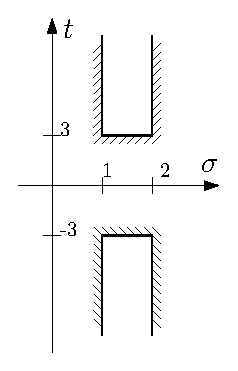
\includegraphics[scale=1.0]{0401}
  \end{wrapfigure}

  \pt{1}
  $$
    \hm{\sum_{n=1}^N\frac1{n^s}}=O(N^\ep)=C_1N^\ep\le C_1|t|^\ep.
  $$

  \pt{2} Имеем $|1-s|=|(1-\si)-it|=\sqrt{(1-\si)^2+t^2}\ge\sqrt{0+4}=2,$ и тогда
  $$
    \hm{\frac{N^{1-s}}{1-s}}\le\frac{N^{1-\si}}{|1-s|}\le\frac{|t|^\ep}2.
  $$

  \pt{3} Используя $|t|-1<N\le|t|$, получаем
  \begin{mlc*}
    \hm{s\intlim_N^\infty\frac{\bc{x}}{x^{s+1}}\,dx} \le
    \sqrt{t^2+9}\intlim_N^\infty\frac{dx}{x^{2-\ep}} \le
    (|t|+3)\left.\frac{x^{\ep-1}}{\ep-1}\right|_N^\infty = \\
    = (|t|+3)\frac{N^\ep N^{-1}}{1-\ep}\le\frac1{1-\ep}\frac{|t|+3}{|t|-1}|t|^\ep \le
    C_2|t|^\ep.
  \end{mlc*}

  Из \pt{1}--\pt{3} следует требуемое.

  Для $\ze'(s)$ воспользуемся формулой Коши:
  $$
    \ze'(s)=\frac1{2\pi i}\intlim_{|z-s|=\ep}\frac{\ze(z)}{(z-s)^2}\,dz,
  $$
  откуда получаем оценку
  %\footnotemark\footnotetext{Почему?}
  $$
    |\ze'(s)|\le\frac1{2\pi}\frac{C_1(|t|+\ep)^\ep}{\ep^2}\le C_2|t|^\ep.
  $$
\end{proof}

Займемся получением такой же оценки для $\frac{\ze'(s)}{\ze(s)}$.

\subsubsection{Лемма о том, что некоторое выражение по модулю не больше $1$}

\begin{lemma}
  При $0<r<1,\,\ph\in\R$
  $$
    M:=\bm{(1-r)^3(1-re^{i\ph})^4(1-re^{2i\ph})}\leqslant1.
  $$
\end{lemma}
\begin{proof}
  \begin{mlc*}
    \ln{M}=3\ln{(1-r)}+4\ln{\bm{1-re^{i\ph}}}+\ln{\bm{1-re^{2i\ph}}}=\\
    =\Re\left(3\ln{(1-r)}+4\ln{(1-re^{i\ph})}+\ln{(1-re^{2i\ph})}\right)=
    -\Re\left(\sum_{n=1}^\infty\frac{r^n}n\left(3+4e^{in\ph}+e^{2in\ph}\right)\right)=\\
    =-\sum_{n=1}^\infty\frac{r^n}n\left(3+4\cos{n\ph}+\cos{2n\ph}\right)=
    -\sum_{n=1}^\infty\frac{r^n}n\cdot2(1+\cos{n\ph})^2\leqslant0.
  \end{mlc*}
  Потенцируя, получаем требуемое.
\end{proof}

\begin{lemma}
  При $\si>1,\,t\in\R$ $$A:=\hm{\ze^3(\si)\ze^4(\si+it)\ze(\si+2it)}\ge1.$$
\end{lemma}
\begin{proof}
  Воспользуемся формулой Эйлера для $\ze(s)$. Тогда получим
  $$
    A=\prod_p\bbbm{\left(1-\frac1{p^\si}\right)^3\left(1-\frac1{p^{\si+it}}\right)^4\left(1-\frac1{p^{\si+2it}}\right)}^{-1}.
  $$

  Выбирая $r:=\frac1{p^\si},\,e^{i\ph}:=p^{-it}$, т.е. $\ph:=-t\ln{p}$, получаем по предыдущей лемме требуемое.
\end{proof}

\subsubsection{Отсутствие нулей $\ze(s)$ в области $\{\si\ge1\}$}

\begin{theorem}
  При $\si\ge1$ $\ze(s)\neq0$.
\end{theorem}
\begin{proof}
  Наше утверждение при $\si>1$ вытекает из последней леммы: если $\ze(s)=0$, то $A=0\ge1$~— противоречие.

  Случай $\si=1$ несколько сложнее.

  Допустим, $\ze(1+it)=0$. Будем считать, что $1<\si<2$.

  \pt{1} Из оценки~(\ref{zeta <= sigma/(sigma-1)})~имеем $0<\ze(\si)\leqslant\frac{\si}{\si-1}<\frac2{\si-1}$.

  \pt{2} В силу непрерывности $\ze(s)$ по $\si$ на $[1;2]$ имеем $|\ze(\si+2it)|\leqslant C_1$.

%   \pt{3} $\ze'(s)=\:?$\footnote{И чему же равно $\ze'(s)$?}, значит, $\limlim_{\si\to1+0}\frac{\ze(\si+it)-\ze(1+it)}{\si-1}=\limlim_{\si\to1+0}\frac{\ze(\si+it)}{\si-1}$, откуда
%   следует, что $\left|\frac{\ze(\si+it)}{\si-1}\right|\leqslant C_2$, т.е. $|\ze(\si+it)|\leqslant C_2|\si-1|$.

  \pt{3} 
	%$\ze'(s)=\:?$\footnote{И чему же равно $\ze'(s)$?}, значит
  $$
    \limlim_{\si\to1+0}\frac{\ze(\si+it)-\ze(1+it)}{\si-1} = \limlim_{\si\to1+0}\frac{\ze(\si+it)}{\si-1} \Rightarrow
    \left|\frac{\ze(\si+it)}{\si-1}\right|\leqslant C_2 \Rightarrow
    |\ze(\si+it)|\leqslant C_2|\si-1|.
  $$

  Тогда
%\footnote{Разъяснить пункты 2, 3.}
  $$
  1\le A\le\left|\left(\frac2{\si-1}\right)^3(C_2(\si-1))^4C_1\right|=C_3|\si-1|\xra{\si\to1+0}0
  $$
  Полученное противоречие доказывает теорему.
\end{proof}

\subsubsection{Оценка для $-\ze'(s)/\ze(s)$}

\begin{theorem}
  В области $D:=\{1\leqslant\si\leqslant2,\,|t|\ge3\}$ $\frac{\ze'(s)}{\ze(s)}$ есть $O(|t|^\ep)$.
\end{theorem}

% \begin{wrapfigure}{r}{120pt}
%   \begin{center}
%   \vskip -50pt
%   \includegraphics[scale=1.0]{0402}
%   \vskip 10pt
%   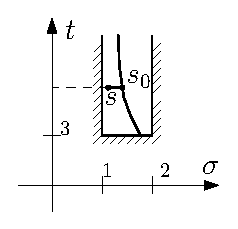
\includegraphics[scale=1.0]{0403}
%   \end{center}
% \end{wrapfigure}

\begin{proof}
  \begin{wrapfigure}{r}{120pt}
    \vskip -40pt
    \includegraphics[scale=1.0]{0402}
  \end{wrapfigure}

  Разобьем нашу область на две части $D_1,\,D_2$ по кривой $\si=1+\la|t|^{-\ep}, \la$ определим позднее.

  \pt{1} Пусть $s\in D_1$. По доказанному можем считать, что $|\ze(\si+2it)| \bw\leqslant C_1|t|^{\ep/5}$. Тогда из леммы имеем
  \begin{mlc*}
    |\ze(s)|=|\ze(\si+it)|\ge\ze(\si)^{-3/4}|\ze(\si+2it)|^{-1/4}\ge\\\ge
    \left(\frac2{\la|t|^{-\ep}}\right)^{-3/4}\left(C_1|t|^{\ep/5}\right)^{-1/4}=\widetilde{C_1}\la^{3/4}|t|^{-{4\ep}/5}.
  \end{mlc*}

  \pt{2} Пусть $\si+it=s\in D_2$. Определим $\si_0(t):=1+\la|t|^{-\ep},\,s_0(t):=\si_0(t)+it$.
  Тогда $\intlim_\si^{\si_0}\ze'(x+it)\,dx\bw=\ze(\si_0+it)-\ze(\si+it).$ Заметим, что выполняется оценка
  $\left|\intlim_\si^{\si_0}\ze'(x+it)\,dx\right|\bw\leqslant(\si_0\bw-\si)C_2|t|^{\ep/5}\leqslant\widetilde{C_2}\la|t|^{-\ep}|t|^{\ep/5}=\widetilde{C_2}\la|t|^{-4\ep/5}.$

  \begin{wrapfigure}{r}{120pt}
    \vskip -50pt
    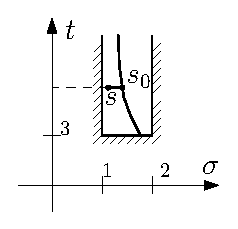
\includegraphics[scale=1.0]{0403}
  \end{wrapfigure}

  Имеем
  \begin{mlc*}
    |\ze(s)|=|\ze(\si+it)|\ge|\ze(\si_0+it)|-\left|\intlim_\si^{\si_0}\ze'(x+it)\,dx\right|\ge \\
    \ge \widetilde{C_1}\la^{3/4}|t|^{-4\ep/5}-\widetilde{C_2}\la|t|^{-4\ep/5}=
    \la^{3/4}\left(\widetilde{C_1}-\widetilde{C_2}\la^{1/4}\right)|t|^{-4\ep/5}.
  \end{mlc*}

  Можем выбрать $\la\colon\widetilde{C_1}-\widetilde{C_2}\la^{1/4}>0.$ Тогда во всей области $D$
  $$
    |\ze(s)|\ge C_3|t|^{-4\ep/5}.
  $$

  Получаем требуемое $$\left|\frac{\ze'(s)}{\ze(s)}\right|\leqslant\frac{C_4|t|^{\ep/5}}{C_3|t|^{-4\ep/5}}=C|t|^\ep.$$
\end{proof} 

\newlecture{5}{29.09.2010}
%$$\zeta (s) = \sum\limits_{n=1}^{\infty} \frac{1}{n^s},\,s = \sigma + it$$
%сходится при $\sigma > 1$
%$$-\frac{\zeta '(s)}{\zeta (s)} = O(\sqrt{t})$$
%при $\sigma > 1$ существует разложение
%$$-\frac{\zeta '(s)}{\zeta (s)} = \sum\limits_{n=1}^{\infty}\frac{\Lambda (n)}{n^s}$$
%где
%$$
%  \Lambda (n) =
%  \begin{cases}
%    \ln p, &n = p^k \\
%    0, &\text{иначe}
%  \end{cases}
%$$
%$$\psi(x) = \sum\limits_{n\leqslant x} \Lambda (n)$$
%Задача~--- доказать асимптотический закон $\pi (x) \sim \frac{x}{\ln x}$, что означает
%$$\lim\limits_{x \rightarrow + \infty} \frac{\pi (x) \ln x}{x}=1.$$\par
%Напомним, что
%$$\pi (x) \sim \frac{x}{\ln x} \Leftrightarrow \psi(x) \sim x, x\rightarrow + \infty,$$где
%$$\omega (x) = \int\limits_1^x \frac{\psi(t)}{t}\,dt$$
\subsection{Асимптотический закон}
\subsubsection{Функция $\om(x)$. Достаточность эквивалентности $\om(x)\sim x$ 
							для доказательства асимптотического закона}

Напомним, что мы доказали совпадение верхних и нижних пределов у функций 
$\frac{\psi(x)}{x}$ и $\frac{\pi(x)\ln{x}}{x}$, поэтому для доказательства
асимптотического закона $\pi(x)\sim\frac{x}{\ln{x}}$ достаточно показать,
что $\psi(x)\sim~x$.

Введем функцию 
$$
	\om(x):=\intlim_1^x \frac{\psi(t)}t\,dt.
$$

\begin{stm}
Если $\omega(x) \sim x$, то $\psi(x) \sim x$.
\end{stm}
\begin{note}
Верно и обратное утверждение, но нам достаточно этого.
\end{note}
\begin{proof}
Возьмем $u > v \geqslant 1$ и рассмотрим
$$
	\int\limits_v^u \frac{\psi(t)}{t}\,dt =\omega(u) - \omega(v) = 
	u - v + o(u) + o(v).
$$

Оценим его грубо сверху и снизу:
$(u-v)\frac{\psi(v)}{u} \leqslant \int\limits_v^u \frac{\psi(t)}{t}\,dt 
\leqslant (u-v)\frac{\psi(u)}{v}.$

Рассмотрим две ситуации:
\begin{points}{0}
\item Выберем $v = x,\,u = (1+\ep)x$, тогда имеем 
	$\ep x\frac{\psi(x)}{(1+\ep)x} \leqslant \ep x + o(x),$
	откуда $\psi(x) \leqslant (1+\ep)x + o(x)$, и найдется $x_1$ такой, 
	что при $x>x_1$ $\psi(x)\le(1+2\ep)x$.

\item Теперь возьмем $u = x,\,v = (1 - \ep)x$ и используем правую оценку: 
	$\ep x + o(x) \le \ep x\frac{\psi(x)}{(1-\ep)x}$, откуда аналогично \pt{1} 
	получаем, что при $x>x_2$ $\psi(x)\ge(1-2\ep)x$.

	Таким образом, при $x>\max{(x_1,\,x_2)}$ имеем
	$$
		1 - 2\ep \le \frac{\psi(x)}{x} \le 1 + 2\ep,
	$$
	откуда очевидно следует утверждаемое.
\end{points}
\end{proof}

Таким образом, асимптотический закон следует из эквивалентности $\om(x)\sim x$.
Наша цель~—~ доказать ее.

\begin{stm} Для $\om(x)$ справедливо равенство
$$\omega(x) = \sum\limits_{n\leqslant x} \Lambda(n) \ln\frac{x}{n}.$$
\end{stm}
\begin{proof}
Прямое применение преобразования Абеля (лемма \ref{abel}).\par
В нашем случае $a_n = \Lambda(n),\,g(t) = \ln\frac{x}{t} = \ln x - \ln t$, тогда $A(x) = \psi(x)$, и получаем
$$\sum\limits_{n\leqslant x} \Lambda(n)\ln\frac{x}{n} = \psi(x)\ln\frac{x}{x} - \int\limits_1^x \psi(t)\left(-\frac{1}{t}\right)dt = \int\limits_1^x \frac{\psi(t)}t\,dt,$$ что и требовалось.
\end{proof}

\subsubsection{Интегральная связь $\om(x)$ и $\ze(s)$}

\begin{lemma} При $a>0,\,b>0$ имеем место соотношение
$$I = \frac{1}{2\pi i}\int\limits_{a - i\infty}^{a + i\infty} \frac{b^s}{s^2}\,ds =
\begin{cases}
\ln b,&b \geqslant 1\\
0,&0<b<1
\end{cases}$$
\center{$\displaystyle s=\si+it$}
\label{lemma_for_om_formula}
\end{lemma}
\begin{proof}
Интеграл абсолютно сходится, потому как  $\left|\dfrac{b^s}{s^2}\right| \leqslant \dfrac{b^a}{a^2 + t^2}$.


%\begin{wrapfigure}[8]{r}{50pt}
%\includegraphics[scale=1]{05011}
%\end{wrapfigure}\par
Наш интеграл $I$ есть предел интегралов от $a-iu$ до $a+iu$, которые вычислим как интегралы по контуру, предварительно его замкнув.\par
\pt{1} Рассмотрим первый случай $b\ge1$. Замыкаем контур той частью окружностью радиуса $\sqrt{u^2 + a^2}$, которая лежит в левой полуплоскости относительно прямой $\Re{z}=a$.\par
\begin{wrapfigure}{r}{80pt}
\begin{center}
\vskip -20pt
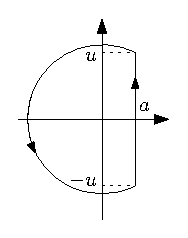
\includegraphics[scale=1.0]{05012}
Случай $b\ge1$
\end{center}
\end{wrapfigure}\par
Получаем:
$$I_0(u)=\frac{1}{2\pi i}\int\limits_{\Gamma(u)} \frac{b^s}{s^2}\,ds = \res_{s = 0}\frac{b^s}{s^2} = \res_{s=0}\frac{1+s\ln b + \ldots}{s^2} = \ln{b}.$$\par
С другой стороны,
$$I_0(u) = \underbrace{\frac{1}{2\pi i}\int\limits_{a - iu}^{a + iu}\frac{b^s}{s^2}\,ds}_{I_1(u)} +
\underbrace{\frac{1}{2\pi i}\int\limits_{\Gamma_1(u)}\frac{b^s}{s^2}\,ds}_{I_2(u)},$$
где $\Gamma_1$~— дуга окружности.\par
Очевидно, $I_1(u)\xra{u\to\infty}I$.\par
Осталось проверить, что второй интеграл стремится к нулю:
$$|I_2(u)| \leqslant \frac{2\pi\sqrt{a^2 + u^2}}{2\pi}\frac{b^a}{a^2 + u^2}\xrightarrow{u \to \infty} 0.$$\par
\begin{wrapfigure}{r}{80pt}
\begin{center}
\vskip -30pt
\includegraphics[scale=1.0]{05013}
Случай $0 < b < 1$
\end{center}
\end{wrapfigure}
\pt{2} При $0 < b <1$ замыкаем контур частью той же окружности, только лежащей в правой полуплоскости.\par
Ни внутри области, ограничиваемой контуром интегрирования, ни на самом контуре подынтегральная функция особых точек не имеет, поэтому
$$\hat{I_0}(u) = \frac{1}{2\pi i}\int\limits_{\hat{\Ga}(u)} \frac{b^s}{s^2}\,ds = 0.$$\par
Вместе с тем ($\hat{\Ga}_1$~— дуга окружности) $$\hat{I_0}(u)=\frac{1}{2\pi i}\int\limits_{a - iu}^{a + iu}\frac{b^s}{s^2}\,ds+
\frac{1}{2\pi i}\int\limits_{\hat{\Ga}_1(u)}\frac{b^s}{s^2}\,ds,$$
и аналогично первому пункту первый интеграл сходится к $I$, а второй~— к $0$.
\end{proof}
\begin{stm}
Для $\om(x)$ при $x\ge2$ верна формула
$$\om(x)=\frac{1}{2\pi i}\int\limits_{2 - i\infty}^{2 + i\infty}\left(-\frac{\zeta '(s)}{\zeta(s)}\right) \cdot \frac{x^s}{s^2}\,ds.$$
\end{stm}
\begin{note}
Именно этим и удобна функция $\om(x)$~— в аналогичной формуле для $\psi(x)$ в знаменателе стоит $s$ не во второй, а в первой степени, что влечет за собой отсутствие абсолютной сходимости интеграла и, таким образом, необходимость рассматривать главное значение, интегрировать не по всей прямой, что неизбежно выливается в значительные технические сложности.
\end{note}
\begin{proof}
Действовать будем так:
$$I = \frac{1}{2\pi i}\int\limits_{2 - i\infty}^{2 + i\infty} \left(\sum\limits_{n=1}^{\infty} \frac{\Lambda(n)}{n^s}\right) \frac{x^s}{s^2} \,ds\eqvl{I}{10} \sum\limits_{n=1}^{\infty} \Lambda(n) \frac{1}{2\pi i} \int\limits_{2 - i\infty}^{2 + i\infty} \frac{(\frac{x}{n})^s}{s^2}\,ds \eqvl{II}{10}\sum\limits_{n\leqslant x} \Lambda(n) \ln\frac{x}{n} = \omega(x).$$\par
Нужно обосновать два равенства~— I и II.\par
\pt{1} С I все просто~— мы меняем здесь местами сумму и интеграл, и действительно можем это делать, потому как
$$\left|-\frac{\zeta '(s)}{\zeta (s)} \cdot\frac{x^2}{s^2}\right| \leqslant \frac{C\sqrt{t} x^2}{t^2 + 4},$$
откуда и следует необходимая нам абсолютная сходимость интеграла.

\begin{note}
У подобной оценки для функции $\psi$ в знаменателе стоит $\sqrt{t^2+4}$, поэтому абсолютная сходимость отсутствует.\par
\end{note}\par
\pt{2} Разберемся с II. Выберем $N > x$ и разобьем сумму на две:
$$\sum\limits_{n=1}^{\infty} \Lambda(n) \frac{1}{2\pi i} \int\limits_{2 - i\infty}^{2 + i\infty} \frac{(\frac{x}{n})^s}{s^2}\,ds
=\sum\limits_{n=1}^{N}\ldots + \underbrace{\sum\limits_{n=N+1}^{\infty}\ldots}_{R_N(s)}\eqvl{\text{лемма }\ref{lemma_for_om_formula}}{40}\om(x)+R_N(s).$$\par
Остается показать, что $R_N(s)\xra{n\to\infty}0$.\par
Вернем сумму под интеграл:
$ R_N(s) = \frac{1}{2\pi i}\int\limits_{2 - i\infty}^{2 + i\infty} \left(\sum\limits_{n = N + 1}^{\infty} \frac{\Lambda(n)}{n^s}\right) \frac{x^s}{s^2}\,ds,$ получаем оценку
$$|R_N(s)| \leqslant \frac{1}{2\pi}\left(\sum\limits_{n = N + 1}^{\infty}\frac{\ln n}{n^2}\right) x^2 \left(\int\limits_{-\infty}^{+\infty} \frac{dt}{t^2 + 4}\right) = \frac{x^2}{2\pi} \frac{\pi}{2} \sum\limits_{n = N+1}^{\infty} \frac{\ln n}{n^2} \xrightarrow{N\to\infty} 0.$$
\end{proof}\par

Хотим показать, что $\omega(x) \sim x$. Грубо оценивая, имеем 
$\omega(x) < Cx^2$ ($Cx^{1+\ep}$, если устремим прямую интегрирования 
к $1$)~— в любом случае хуже тривиальной оценки $\omega(x) < x\ln ^2 x$.

%\begin{note}
%С этого места лучше читать книгу Галочкина в районе 45 страницы. Когда-нибудь с учетом этого мы приведем лекцию в порядок.
%\end{note}

\subsubsection{Выделение главного члена в интегральной формуле для $\om(x)$}

Нужно, чтобы значительная часть интеграла проходила левее $\Re s=1$. Выберем путь интегрирования $\Gamma(\eta, T)$, зависящий от двух параметров $T,\,T>0$ и $\eta,\,0<\eta<1$, значение которых подберем уже по ходу доказательства.\par
\begin{wrapfigure}{r}{80pt}
\begin{center}
\vskip -20pt
\includegraphics[scale=1.0, trim=20 0 0 0]{05021}
\end{center}
%\caption{Область интегрирования}
\end{wrapfigure}
\begin{stm} Если в заштрихованной области $\zeta(s) \not = 0$, то
$$\omega(x) = x(1 + R(x))$$ где $$R(x) = \frac{1}{2\pi i} \int\limits_{\Gamma(\eta, T)} \left(-\frac{\zeta '(s)}{\zeta (s)}\right)\frac{x^{s-1}}{s^2}\,ds.$$
\end{stm}
\begin{proof}
\begin{wrapfigure}{r}{100pt}
\begin{center}
\includegraphics[scale=1.0, trim=20 0 0 0]{05022}
\end{center}
%\caption{Область интегрирования}
\end{wrapfigure}

Будем рассматривать интегралы по контуру $\Ga_0(\eta,T,u)$. Заметим, что 
в пределе (при $u\to\infty$) интеграл от функции $-\frac{\zeta '(s)}{\zeta 
(s)} \frac{x^s}{s^2}$ по пути $ABCDEF$ дает нам $-xR(x)$, а по пути $GH$~—
$\om(x)$. Сейчас мы докажем, что интеграл по всему контуру $\Ga_0$ равен $x$, 
затем~— что интегралы по перемычкам $FG$ и $HA$ равны $0$, откуда, переходя 
к пределу, получим равенство $x = \om(x) - xR(x)$.

Действительно, рассмотрим
$$I_0(u):=\frac{1}{2\pi i} \int\limits_{\Gamma_0(\eta,T,u)}
\left(-\frac{\zeta '(s)}{\zeta (s)}\right)\frac{x^{s}}{s^2}\,ds = 
\res_{s=1} \left(-\frac{\zeta '(s)}{\zeta (s)}\right)\frac{x^s}{s^2}
\eqvl{$(*)$}{10}x.$$

Почему верен переход $(*)$? Как мы знаем (формула $(\ref{36})$), $\ze(s)$ 
представима в виде $\zeta(s) \bw= \frac{1}{s-1} + f(s)$, где $f$~— 
аналитическая в области $\sigma > 0$, тогда
$$-\frac{\zeta '(s)}{\zeta (s)} = -\frac{-1/(s-1)^2 + f'(s)}{1/(s-1) + f(s)} = 
\frac{1}{s-1}\frac{1 - (s-1)^2f'(s)}{1 + (s-1)f(s)},$$
откуда следует, что функция $-\frac{\zeta '(s)}{\zeta (s)} \frac{x^s}{s^2}$
имеет в нашей области единственную особую точку $s=1$, вычет в которой равен 
$x$.

Остается показать, что интеграл по перемычкам $FG$ и $HA$ стремится к нулю 
при $u\to\infty$:
$$\left|\mp\frac{1}{2\pi i} \int\limits_{1 \pm iu}^{2\pm iu}
\left(-\frac{\zeta '(s)}{\zeta (s)}\right)\frac{x^s}{s^2}\,ds\right| \leqslant
\frac{1}{2\pi}\cdot 1\cdot c\sqrt{u}\cdot\frac{x^2}{u^2} \xra{u\to\infty} 0.$$

Значит, $\limlim_{u\to\infty}I_0(u) =x= \omega(x) - xR(x)$.
\end{proof}

\subsubsection{Доказательство асимптотического закона}

\begin{theorem}[Асимптотический закон]
%$$\lim\limits_{x\to+\infty} \frac{\pi(x) \ln(x)}{x} = 1$$
При $x\to+\infty$ 
$$
	\pi(x)\sim \frac{x}{\ln{x}}.
$$
\end{theorem}
\begin{wrapfigure}{r}{80pt}
\begin{center}
%\vskip 20pt
\includegraphics[scale=1.0, trim=20 0 0 0]{05024}
\end{center}
\end{wrapfigure}
%\vskip 20pt
\begin{proof}
Теперь нам достаточно доказать, что $\lim\limits_{x\to+\infty} R(x) = 0$.\par
Имеем $R(x) = I_1(x) + I_2(x) + I_3(x) + I_4(x) + I_5(x)$.\par
Сначала выбираем $T \geqslant 3$. Начнем оценивать с $I_1(x) = \frac{1}{2\pi i} \int\limits_{1 + iT}^{1 + i\infty} \left(-\frac{\zeta '(s)}{\zeta (s)}\right)\frac{x^{s-1}}{s^2}\,ds.$\par
Заметим, что $|x^{s-1}| = |x^{it}| = 1$, значит, оценка имеет вид:
$$|I_1(x)| \leqslant \frac{1}{2\pi} \int\limits_T^{+\infty} \frac{c\sqrt{t} }{1 + t^2}\cdot1\,dt < \frac{\ep}5,\text{ где }T > T_0(\ep).$$\par
Аналогично $|I_5(x)| < \ep/5$.

%\begin{wrapfigure}{r}{80pt}
%\begin{center}
%\vskip -10pt
%\includegraphics[scale=1.0, trim=20 0 0 0]{05023}
%Ука\-зан\-ная область
%\end{center}
%\end{wrapfigure}
У аналитической функции $\ze(s)$ в заштрихованной области $BCDE$ конечное число
нулей: в противном случае они имеют предельную точку, и $\ze(s)\equiv0$. 
Выберем $\eta$ как половину расстояния от $\{\si=1\}$ до ближайшего нуля.

Заметим, что благодаря такому выбору $\eta$ функция
$\left|-\frac{\zeta '(s)}{\zeta (s)} \frac{1}{s^2}\right|$ непрерывна на 
$BCDE$. Тогда найдется такая константа $M=M(T,\eta)$, что
$$\left|-\frac{\zeta '(s)}{\zeta (s)} \frac{1}{s^2}\right| \leqslant M.$$

Оценим еще пару интегралов. Рассмотрим
$I_2(x) = \frac{1}{2\pi i}\int\limits_{\eta + iT}^{1 + iT} 
\left(-\frac{\zeta '(s)}{\zeta (s)}\right) \frac{x^{s-1}}{s^2}\,ds.$ 
Для него верна оценка
$$|I_2(x)| \le \frac{1}{2\pi}\int\limits_{\eta}^{1} M x^{\si -1}\,d\si \le
\frac{1}{2\pi}\int\limits_{-\infty}^{1} M x^{\sigma -1}\,d\sigma = 
\frac{1}{2\pi}\frac{M}{\ln x} \xra{x\to\infty} 0.$$

Значит, $|I_2(x)| < \ep/5,\,|I_4(x)| < \ep/5$ при $x > x_1(\ep)$.\par
Остался последний шаг. Рассматриваем $I_3(x) = \frac{1}{2\pi i}\int\limits_{\eta - iT}^{\eta + iT} \left(-\frac{\zeta '(s)}{\zeta (s)}\right)\frac{x^{s-1}}{s^2}\,ds,$ и тогда
$$|I_3(x)| \leqslant \frac{1}{2\pi}M\cdot 2T\cdot x^{\eta-1} < \ep/5$$
при $x > x_2(\ep)$, потому как $\eta - 1 < 0$.\par
Таким образом, при $x > \max( x_1(\ep),\, x_2(\ep))$ и $T > T_0(\ep)$ получаем $$|R(x)| < \ep.$$
\end{proof}
\begin{imp}
При $n\to\infty$ $P_n \sim n\ln n$.
\end{imp}

\newlecture{6}{06.09.2010}

Таким образом, $\pi(x)=\frac{x}{\ln x}+R(x)$, $R(x)$ есть 
$o\left(\frac{x}{\ln x}\right)$. Если постараться, можно показать, что 
$R(x)\bw=O\left(\frac{x}{\ln^2x}\right)$, но не более того.	

\subsubsection{Следствия асимптотического закона}

Отметим важное следствие.
\begin{imp}
  $p_n \sim n \ln n$
\end{imp}
\begin{proof}
  Имеем $\pi(p_n) = n = \dfrac{p_n}{\ln p_n} (1 + o(1))$. 

	Прологарифмируем, получим: $\ln n = \ln p_n - \ln\ln p_n + \ln (1 + o(1))$. 

	Теперь перемножим	эти равенства: 
	$$
		n \ln n = \frac{p_n}{\ln p_n} (1 + o(1))(\ln p_n - \ln\ln p_n
	 + \ln(1 + o(1))) \sim p_n.
	$$
\end{proof}

Очевидно, $\ln[1,2,\dots,n] = \psi(n) \sim n$, откуда получаем еще одно
\begin{imp}
	$[1,2,\dots,n] = e^{n(1+o(1))}$.
\end{imp}

\subsubsection{Интегральный логарифм и нерешенные задачи}

Оказывается, $\pi(x)$ лучше приближает \notion{интегральный логарифм}: 
$$\li x = \int\limits_2^x\frac{dt}{\ln t},$$ и для функции $R(x)$ в этом 
случае можно добиться гораздо лучших оценок.

Очевидно, по правилу Лопиталя
$\lim\limits_{x\to+\infty} \frac{\li x}{x}\ln x = 1$. Рассмотрим 
$\pi(x)=\li x+R(x)$. Используя то, что $\ze(s)$ не обращается в $0$ в
$\{\si>1-\frac{c}{\ln t}\}$, можно доказать (что и было сделано Вале-Пуссеном),
что $$R(x)<xe^{-c\sqrt{\ln x}}<\frac{x}{(\ln x)^c}\,\text{ для любого } c>1.$$

Лучшая известная на данный момент оценка (Виноградов, Коробов, 1959 год) для
функции $R(x)$: $$R(x)<xe^{-c(\ln x)^{3/5-\ep}}.$$

При этом, если верна гипотеза Римана о том, что все нетривиальные нули 
$\ze$-функции лежат на прямой $\si=\frac12$, то для $R(x)$ выполняется куда 
более сильная оценка: $$R(x)<\sqrt{x}\ln x.$$

В 30-е годы было доказано, что $\pi(x) - \li x $ бесконечное число раз меняет 
знак, хотя во всех известных таблицах $\pi(x) < \li x$.

С простыми числами связано множество нерешенных задач. Среди них~— проблема 
Эйлера-Гольдбаха: правда ли, что любое нечетное натуральное число $n>8$
представимо в виде суммы трех простых. Виноградов доказал, что это верно для 
достаточно больших $n$ ($n>N$, где $N\sim10^{20}$). 

Известно также предположение Эйлера о том, что всякое четное число представимо
в виде суммы двух простых. Пока что доказано лишь, что 
$$\frac{\Card\{\text{все четные, непредставимые в таком виде}< n\}}
{\Card\{\text{все натуральные числа}< n\}}\xra{n\to\infty}0.$$

\section{Теорема Дирихле о бесконечном количестве простых чисел в 
				арифметических прогрессиях}

	Цель этого раздела~— доказательство открытой Дирихле в 1839 году теоремы, 
	гласящей, что в любой арифметической прогрессии,
	первый член и разность которой~— взаимно простые натуральные числа, 
	содержится бесконечно много простых чисел.

Стоит отметить, что, хотя задача для арифметических прогрессий была
решена более полутора веков назад, до сих пор неизвестно, бесконечно ли много
простых чисел в последовательности чисел вида, например, $n^2+1$.
	
% Среди $mx + a, (a,m) = 1$ содержится бесконечно много простых чисел~— доказано Дирихле в 1839 году. Нужно доказать бесконечность множества простых чисел, удовлетворяющих сравнению $ p = a \pmod m$.

\subsection{Сравнения и их свойства}

\subsubsection{Определение сравнений, элементарные свойства}

\begin{df}
Говорят, что числа \notion{$a$ и~$b$ сравнимы по модулю~$m$}, если они дают 
одинаковые остатки при делении на $m$.
\end{df}

Здесь $a$ и $b$~— целые числа, $m$~— натуральное, не меньшее $2$.
\begin{denote}
$a \eq b \pmod m$.
\end{denote}

Справедливо следующее очевидное утверждение.
\begin{stm}
Числа $a$ и~$b$ сравнимы по модулю~$m$ тогда и только тогда, когда $m \divs a-b$.
\end{stm}

Имеют место свойства:
\begin{points}{0}
  \item $a \eq b \pmod m \llra b \eq a \pmod m$\par
  \item $a \eq b \pmod m \llra a+c \eq b+c \pmod m$\par
  \item $a \eq b \pmod m \lRa ac \eq bc \pmod m$\par
  \item $a \eq b \pmod m,\:c \eq d \pmod m \lRa a + c \eq b + d \pmod m,\:
		ac \eq bd \pmod m$ 
\begin{proof}
	$ac \eq bc \eq bd \pmod m$
\end{proof}
  \item $ac \eq bc \pmod m,\:(c,m) = 1 \lRa a \eq b \pmod m$
\begin{proof}
  $m \divs c(a - b),\,(c,m) = 1 \lRa m \divs a - b$
\end{proof}

	\item $a \eq b \pmod m \llra ac \eq bc \pmod{mc},\,c \neq 0$
\end{points}

\subsubsection{Уравнения в сравнениях, линейные сравнения}

Можно решать уравнения относительно сравнений: 
$a_nx^n + \dots + a_0 \eq 0 \pmod m$. Очевидно, если $x_0$~— решение, то 
весь класс $x \eq x_0 \pmod m$~— решение. Таким образом, количество классов 
вычетов по модулю $m$ и есть количество решений этого сравнения.

Уравнение $a_nx^n + \dots + a_0 \eq 0 \pmod p $ по модулю
простого числа имеет не более $n$ классов решений. Действительно, в этом случае
мы фактически ищем корни многочлена $a_nx^n + \dots + a_0 = 0$ в факторгруппе 
$\Z_p=\fact{\Z}{p\Z}$, которая является полем при простых $p$; в поле же число 
корней многочлена не превышает его степень.

Если $m$ не является простым, то это уже не верно: например, уравнение
$x^2 \eq 1 \pmod 8$ имеет корни $x \eq 1, 3, 5, 7 \pmod 8$.

Рассмотрим линейные сравнения.
\begin{stm}
  Сравнение $ax \eq b \pmod m,\,(a,m)=1$ всегда имеет и ровно одно решение.
\end{stm}
\begin{note}
Условие $(a,m)=1$, понятное дело, никак не ограничивает класс рассматриваемых 
сравнений: если $(a,m)\neq1$, то мы всегда можем сократить на него и
свести к нужному.
\end{note}
\begin{proof}
	Докажем существование. Найдутся целые $u,\,v$: $au+mv=1$, значит, 
	$au\eq1\pmod m$, откуда $abu\eq b\pmod m$.
\begin{note}
Это сразу же дает нам и алгоритм решения~— алгоритм Евклида.
\end{note}
	Покажем единственность. Действительно, пусть найдутся два решения 
	$ax_1\eq b\pmod m$, $ax_2\eq b\pmod m$. Тогда $a(x_2-x_1)\eq0\pmod m$. Но
	$a$ взаимнопросто с $m$, значит (\pt 5), $x_2-x_1\eq0\pmod m$.
\end{proof}

\subsubsection{Группы $\Z_m$ и $\Z_m^*$}

Пусть $m \geqslant 2$~— натуральное число. Тогда определена факторгруппа 
$\Z_m = \fact{\Z}{m\Z}=\{\overline{a}: a + mt, t \in \Z \}$ с операциями на
классах $\overline{a+b} = \overline{a} + \overline{b},\,
\overline{a\cdot b} = \overline{a} \cdot \overline{b}$

Очевидно, $\Z_m$~— группа по сложению при любом $m$, $\Z_m\setminus\{0\}$
~— группа по умножению тогда и только тогда, когда $m$~— простое: 
в противном случае $m = m_1m_2$, а значит, $\overline{m_1}\cdot\overline{m_2} = 
\overline{0}$.

\begin{df}
$\Z_m^*$ есть набор тех классов из $\Z_m$, которые порождены элементами, 
взаимнопростыми с $m$, то есть 
$\Z_m^* =\{\overline{a}: a + mt,\,t \in \Z,\,(a,m) = 1 \}$.
\end{df}
\begin{stm}
  $\Z_m^*$~— абелева группа по умножению.
\end{stm}
\begin{proof}
  Во-первых, проверим корректность умножения:
  \begin{points}{0}
    \item Если $(a,m) = 1,\, b \eq a \pmod m$, то $(b,m) = 1$. \par
		Действительно, $b = a+mt$, поэтому, если $p \divs b,\,p \divs m$, то 
		$p \divs a$~—противоречие.
    \item Если $(a,m) = 1,\,(b,m) = 1$, то $(ab,m) = 1$. \par
		Предположим, $p \divs ab,\,p \divs m$, тогда $p \divs a$ или $p \divs b$
		~— противоречие.
  \end{points}

  Во-вторых, групповые свойства:
  \begin{points}{0}
    \item Коммутативность и ассоциативность очевидны.
    \item Единица группы есть $\overline{1}$: $\overline{a}\cdot\overline{1}=\overline{a}$.
    \item Для любого элемента группы найдется обратный.\par
		Действительно, доказали, что $ax \eq 1 \pmod m$~— разрешимо. Если $x_0$~— 
		решение, то $\overline{x_0} = \overline{a}^{-1}$.
  \end{points}
\end{proof}

\subsubsection{Функция Эйлера, теорема Лагранжа и следствия}

Нам потребуется один результат из алгебры.

\begin{theorem}[Лагранж]
Пусть группа $G$ конечна, и $H$ — её подгруппа. Тогда порядок $G$ равен порядку 
$H$, умноженному на количество её левых или правых классов смежности.
\end{theorem}

\begin{imp}
Порядок любого элемента конечной группы $G$ делит порядок $G$.
\end{imp}

\begin{proof}
Следует из того, что порядок элемента равен порядку циклической подгруппы, им
порожденной.
\end{proof}

\begin{df}
\notion{Функцией Эйлера} называется 
$\ph(m) = \Card\{x\in\N: 1 \leqslant x \leqslant m,\, (x,m)=1\}$.
\end{df}

Ясно, что $|\Z_m^*| = \varphi(m)$. 
По только что доказанному следствию для любого
$\overline{a}$ из $\Z_m^*$ верно равенство $\overline{a}^{\varphi(m)} 
= \overline{1}$.

Отсюда получаем два важных результата.
\begin{imp}[Теорема Эйлера]
  Для произвольного целого $a$ такого, что $(a,m) =1$, верно $a^{\varphi(m)} 
	\eq 1 \pmod m$.
\end{imp}

\begin{imp}[Малая теорема Ферма]
  Для каждого простого $p$, не делящего $a$, $a^{p-1} \eq 1~\pmod p$.
\end{imp}

\begin{proof}
  В силу очевидного $\ph(p)=p-1$.
\end{proof}

\begin{imp}
В условиях предыдущего следствия $a^p\eq a\pmod p$.
\end{imp}

\subsubsection{Бесконечность количества простых чисел в некоторых частных 
							арифметических прогрессиях}

\begin{lemma}
	\label{p divs a^2+b^2}
  Пусть нечетное простое $p$ делит $a^2 + b^2$, и $(a,b) = 1$. Тогда $p$ имеет 
	вид $4n + 1$.
\end{lemma}

\begin{proof}
  Понятно, $p \ndivs a$ и $p \ndivs b$: иначе $(a,b) \not = 1$. Тогда 
	$a^2 \eq -b^2 \pmod p$. А значит, $a^{p-1} \eq (-1)^{\frac{p-1}{2}} b^{p-1} 
	\pmod p$. С другой стороны, в силу малой теоремы Ферма 
	$a^{p-1}\eq b^{p-1}\eq1\pmod p$, откуда по свойству \pt 5 сравнений 
	$1 \eq (-1)^{\frac{p-1}{2}} \pmod p$. Но $p\geqslant 3$, 
	так что это означает просто $(-1)^{\frac{p-1}{2}} = 1$, а следовательно, 
	$\frac{p-1}{2} = 2n$, то есть $p = 4n + 1$.
\end{proof}

\begin{stm}
  В прогрессии вида $4n - 1,\,n = 1,2,\dots$ содержится бесконечное количество 
	простых чисел.
\end{stm}

\begin{proof}
  Пусть конечное: $p_1,\ldots,p_m$. Рассмотрим $4p_1\dots p_m - 1 = q_1\dots q_s$. 
	Среди $q_j$ есть число вида $4k - 1$, потому как произведение чисел вида 
	$4k + 1$ есть число того же вида. Значит, для некоторого $k$ $q_j=p_k$, тогда
	$p_k \divs 4p_1\dots p_m-1$, откуда $p_k\divs 1$, что невозможно.
\end{proof}

\begin{note}
  Для прогрессии вида $6n - 1$ все аналогично.
\end{note}

\begin{stm}
 В прогрессии вида $4n + 1,\,n = 1,2,\dots$ содержится бесконечное количество 
	простых чисел.
\end{stm}

\begin{proof}
  Пусть конечное: $p_1,\dots,p_m$. Рассмотрим 
	$(2p_1\dots p_m)^2 + 1 = q_1\ldots q_s$. По лемме $(\ref{p divs a^2+b^2})$
	все $q_i=4n_i+1$, поэтому для	некоторого $k$ $q_l=p_k$, значит, 
	$p_k\divs(2p_1\dots p_m)^2 + 1$, откуда	$p_k\divs 1$, чего быть не может.
\end{proof}

\newlecture{7}{13.10.2010}
\subsection{Мультипликативные функции и формула обращения}
\subsubsection{Основные определения}

\begin{df}
Функция $f$ называется \notion{арифметической}, если она действует из $\N$ в
$\Cbb$, и $f \not \equiv 0$. 
\end{df}

\begin{note}
Иногда арифметической называют $f\colon\Z\to\Cbb$.
\end{note}

\begin{df}
Арифметическая $f$ называется \notion{мультипликативной}, если $f(nm) = f(n)f(m)$ для 
всех взаимно простых $n$ и $m$, и \notion{вполне мультипликативной}, если 
$f(nm) = f(n)f(m)$ для всех $n$ и $m$.
\end{df}

По мультипликативной функции $f$ построим другую функцию $F$:
$$
  F(n) = \sum_{d \divs n} f(d).
$$

Очевидно, что, если $n = {p_1}^{k_1} \ldots {p_s}^{k_s}$,
\begin{equation}
	\label{decomposition for multiplicative functions}
  F(n) \eqvl{$I$}{20} \prod_{j=1}^{s} (1 + f(p_j) \spl f({p_j}^{k_j}))
	\eqvl{$II$}{20} \prod_{j=1}^{s} (1 + f(p_j) \spl f({p_j})^{k_j}),
\end{equation}
равенство $I$ верно здесь в случае мультипликативности $f$, равенство $II$~—
в случае вполне мультипликативности.

\begin{df}
\notion{Функцией Мебиуса} называют
$$
\mu(n) = \begin{cases}
    0,& \mbox{если $p^2 \divs n$},\\
    (-1)^k,& \mbox{если $n = p_1 p_2 \ldots p_k$.}
\end{cases}
$$
\end{df}

Она, очевидно, мультипликативна, но не вполне мультипликативна: 
$0=\mu(4)\neq\mu^2(2)=1$.

В силу $(\ref{decomposition for multiplicative functions})$
$$
  \sum_{d \divs n} \mu(d) = 
	\begin{cases}
    1,& \mbox{если $n = 1$,}\\
    0,& \mbox{иначе.}
  \end{cases}
$$

Аналогично считается
$$
  \sum_{d \divs n} \frac{\mu(d)}d = 
	\begin{cases}
		1,& \mbox{если $n = 1$,}\\
		\prodlim_{p \divs n} (1 - \frac1p),& n>1.
	\end{cases}
$$

\subsubsection{Формула обращения Мебиуса}

\begin{theorem}[Формула обращения Мебиуса]
Функция $f$ выражается через $F$ следующим образом
$$
  f(n) = \sum_{d \divs n} \mu(d) \cdot F(n / d).
$$
\end{theorem}
\begin{proof}
	Действительно,
  $$
  \begin{gathered}
  \sum_{d \divs n} \mu(d) \cdot F(n / d) = \sum_{d \divs n} \mu(d) \sum_{d_1 \divs n/d} f(d_1) = \sum_{dd_1 \divs n} \mu(d) \cdot f(d_1)
  = \sum_{d_1 \divs n} f(d_1) \sum_{d \divs n/d_1} \mu(d) = f(n).
  \end{gathered}
  $$
\end{proof}

\subsubsection{Явная формула для функции Эйлера}

Напомним, функцией Эйлера называется $\ph(n)=\Card\{k\mid k\leqslant n,\,(k,n)=1\}$. 
Например, $\ph(p) = p - 1$, $\ph(8) = 4$.

Хотим получить явную формулу для $\ph(n)$, зная разложение $n$ на простые.

Рассмотрим $$A_d:=\{k \mid k \leqslant n, (k, n) = d\} = 
\{k \mid k \leqslant n,\,\left(\frac{k}{d}, \frac{n}{d}\right) = 1\}$$
%center{ $\hm{A_d} = \ph\left(\frac{n}{d}\right)$.}

Ясно, что $ \{1,\dots,n\}=\bigcup_{d\divs n} A_d$, и $\hm{A_d}=\ph(\frac{n}{d})$ поэтому
$$\sum_{d \divs n} \ph(d) = \sum_{d \divs n} \ph(n / d) = \sum_{d \divs n} |A_d| = n.$$

Отсюда уже легко следует

\begin{theorem}
	Для $\ph(n)$ справедливо равенство
  $$
    \ph(n) = n \prod_{p \divs n} \left(1 - \frac1p\right).
  $$
\end{theorem}
\begin{proof}
  Пользуемся формулой обращения Мебиуса:
  $$
    \ph(n) = \sum_{d \divs n} \mu(d) \frac{n}d = 
		n \prod_{p \divs n} \left(1 - \frac1p\right).
  $$
\end{proof}

Заметим, что $\ph$ мультипликативная, но не вполне мультипликативная: 
	$\ph(4) \neq \ph^2(2)$.

Из других свойств $\ph(n)$ можно отметить, например, что 
$$\frac{\ph(1) \spl \ph(n)}n \sim \frac{3}{\pi^2}n.$$

\subsection{Групповые характеры}

\subsubsection{Определение и основные свойства}

Пусть $G$~— конечная абелева группа (операцию будем обозначать умножением), 
$|G| = h$.

\begin{df}
  Характер $\chi$~— это не тождественно нулевой гомоморфизм из $G$ в 
	$(\Cbb, \cdot)$, то есть такой $\chi\colon G\to\Cbb$:
\begin{points}{0}
	\item $\chi(g)\not\eq0$,
	\item $\fa g_1,g_2$ $\chi(g_1g_2)=\chi(g_1)\chi(g_2)$.
\end{points}
\end{df}

Пример: $\chi \equiv 1$~— главный характер.

Свойства характеров:

\pt{1} $\chi(e) = 1$,

	\begin{proof}
		Действительно, найдется $\chi(g)\not\eq0$, тогда $\chi(g)=\chi(ge)=
		\chi(g)\chi(e)$, остается лишь сократить на $\chi(g)$.
	\end{proof}

\pt{2} $\chi(g)^{\ord{g}} = 1$

	\begin{proof}
		Очевидно: $\chi(g)^{\ord g}=\chi(g^{\ord g})=\chi(e)=1$.
	\end{proof}     

	\begin{imp}
	Для любого элемента $g$ из $G$ $\chi(g)^h=1$.
	\end{imp}

	\begin{proof}
	Очевидно в силу того, что для любого элемента группы $\ord g\divs h$.
	\end{proof}

	\begin{imp}
	Все характеры~— комплексные корни из $1$.
	\end{imp}

\pt{3} $\chi(g^{-1}) = 1 / \chi(g)$.

	\begin{proof}
	$\chi(g^{-1})\chi(g)=\chi(g^{-1}g)=\chi(e)=1$.
	\end{proof}

Далее нам понадобится теорема из алгебры:

\begin{theorem}
Любая конечная абелева группа может быть разложена в прямую сумму
\footnote{В нашем случае~— в прямое произведение} своих циклических подгрупп, 
порядки которых являются степенями простых чисел.
\end{theorem}

Таким образом, $$G = G_1 \otimes G_2 \sot G_n,$$
где $G_i=\langle g_i\rangle$~— циклические подгруппы. 
Считаем $g_i$ порядка $h_i$ порождающим элементом $G_i$. Следовательно, каждый 
элемент $g$ представляется в виде $g = {g_1}^{r_1} \sd {g_n}^{r_n}$, 
где $0 \le r_i < h_i$.

Пусть $\zeta_1 \sco \zeta_n$~— корни из единицы степеней $h_1 \sco h_n$. 
Рассмотрим функции вида $$\chi(g) = {\ze_1}^{r_1} \sd {\ze_n}^{r_n}.$$

\pt{4}
  Функции такого вида являются характерами, других характеров нет. Более того, 
	различные $\ze$ дают разные характеры.

\begin{proof}

  \begin{stm}
    Если $g = {g_1}^{k_1} \sd {g_n}^{k_n}$, где $k_i \in \Z$, 
		то $\chi(g) = {\ze_1}^{k_1} \sd {\ze_n}^{k_n}$.
  \end{stm}

  \begin{proof}
	Справедливо $k_j=q_jh_j+r_j,\,0\le r_j < h_j$, и 
	${g_1}^{k_1}\sd{g_n}^{k_n}={g_1}^{r_1}\sd{g_n}^{r_n}$. Тогда $\chi(g)=
	\chi({g_1}^{k_1}\sd{g_n}^{k_n})=\chi({g_1}^{r_1}\sd{g_n}^{r_n})=
	{\ze_1}^{r_1}\sd{\ze_n}^{r_n}={\ze_1}^{k_1}\sd{\ze_n}^{k_n}$.
%    Очевидно, так как $g_i^{h_i} = e$, а $\zeta_i^{h_i} = 1$.
  \end{proof}

	\begin{imp}
  Все $\chi$ такого вида являются характерами.
	\end{imp}

	\begin{proof}
	Пусть $a={g_1}^{k_1}\sd{g_n}^{k_n}$, $b={g_1}^{l_1}\sd{g_n}^{l_n}$.
	Тогда $\chi(ab)={\ze_1}^{k_1+l_1}\sd{\ze_n}^{k_n+l_n}=\chi(a)\chi(b)$.
	\end{proof}
	
	\begin{stm}
	Любой характер имеет такой вид.
	\end{stm}

	\begin{proof}
	Заметим, что $1=\chi(e)=\chi({g_j}^{h_j})=\chi(g_j)^{h_j}$, откуда 
	$\chi(g_j)=\ze_j\colon{\ze_j}^{h_j}=1$.
	\end{proof}

	\begin{stm}
	Разные наборы корней дают разные характеры.
	\end{stm}

	\begin{proof}
	Пусть есть два набора корней из единицы $\ze_1\sco\ze_n$ и 
	$\eta_1\sco\eta_n$, задающие характеры $\chi$ и $\widetilde{\chi}$.
	Без ограничения общности $\ze_1\not=\eta_1$. Тогда $\chi(g_1)=\ze_1\not=
	\eta_1=\widetilde\chi(g_1)$.
	\end{proof}
 	
	Эти утверждения, очевидно, доказывают \pt{4}.
\end{proof}

\begin{imp}
Всего характеров $h_1\sd h_n=h$.
\end{imp}

\begin{imp}
  $G$ изоморфна группе своих характеров.
	\label{G sim character group}
\end{imp}

\begin{problem}
Доказать следствие $\ref{G sim character group}$.
\end{problem}

\begin{stm}
  Пусть $G \ni g \ne e$. Тогда существует характер $\chi$ такой, что 
	$\chi(g) \ne 1$.
\end{stm}

\begin{note}
Грубо говоря, характеров достаточно много, чтобы различать все элементы.
\end{note}

\begin{proof}
  Разложим $g$ по степеням порождающих: $$g = {g_1}^{r_1} \sd {g_n}^{r_n}.$$

  Найдется $r_j\ne0$, поэтому, не умаляя общности, считаем, что $0 < r_1 < h_1$. 
	Возьмем $\zeta_1 = e^{2\pi i / h_1}$, $\zeta_j = 1$ при $j > 1$. Тогда 
	$\chi(g) = e^{2\pi i \cdot r_1 / h_1} \ne 1$.
\end{proof}

%Так как характеры не равны нулю, то легко видеть, что поточечное умножение задает групповую структуру на характерах. Роль единицы играет главный характер.
Определим операцию умножения на характерах естественным образом:
$$\chi_1\chi_2(g)=\chi_1(g)\chi_2(g).$$

\pt{6} Характеры с такой операцией образуют абелеву группу.
\begin{proof}
Сначала проверим, что произведение характеров будет характером. Имеем
$\chi_1 \chi_2 (g_1 g_2) =\linebreak= \chi_1 (g_1 g_2) \chi_2 (g_1 g_2) = 
\chi_1 (g_1) \chi_1 (g_2) \chi_2 (g_1) \chi_2 (g_2) = \chi_1 \chi_2 (g_1) 
\chi_1 \chi_2 (g_2)$.

Главный характер $\chi_0$ будет единицей группы: $\chi\chi_0(g)
=\chi(g)\chi_0(g)=\chi(g)$.

Определим обратный элемент $\chi^{-1}(g):=1/\chi(g)$. Это характер, потому как
$\chi^{-1}(ab)=1/\chi(ab)\bw=1/\chi(a)\cdot1/\chi(b)=\chi^{-1}(a)\chi^{-1}(b).$

Коммутативность и ассоциативность группы следуют из коммутативности и 
ассоциативности $\Cbb$.
\end{proof}

\subsubsection{Два полезных утверждения}

Теперь докажем два полезных равенства.

\begin{stm}
  $$
    S := \sum_{g \in G} \chi(g) = \begin{cases}
      |G|,& \mbox{если $\chi$ главный,}\\
      0,& \mbox{иначе.}
    \end{cases}
  $$
\end{stm}

\begin{stm}
  $$
    \sigma := \sum_{\chi} \chi(g) = \begin{cases}
      |G|,& \mbox{если $g = e$,}\\
      0,& \mbox{иначе.}
    \end{cases}
  $$
\end{stm}

\begin{proof}
  Первые строчки в обоих утверждениях очевидны.

  Докажем вторую строчку первого утверждения. 
	Так как $\chi$ неглавный, то найдется $g_1$ такой, что $\chi(g_1) \ne 1$. 
	$S\cdot\chi(g_1)= \sumlim_{g \in G} \chi(g g_1) 
	= \sumlim_{g \in G} \chi(g) = S$, откуда $S = 0$.

  Докажем вторую строчку второго утверждения. 
	Так как $g \ne e$, то существует $\chi_1$ такой, что $\chi_1(g) \bw\ne 1$. 
	Тогда $\si\cdot\chi_1(g)=\sumlim_\chi\chi\chi_1(g)=\sumlim_\chi\chi(g)=\si$,
	из чего заключаем, что $\sigma = 0$.
\end{proof}


\newlecture{8}{20.10.2010}
\subsubsection{Числовые характеры}

Числовой характер $\chi$ отображает $\Z$ в $\Cbb$. На $\Z_m^*$ он равен групповому характеру, вне $\Z_m^*$~— нулю. Можно дать определение без ссылки на групповые характеры.

\begin{df}
  $\chi \colon \Z \to \Cbb$  называется числовым характером, если
  \begin{enumerate}
    \item Если $x \equiv y \pmod m$, то $\chi(x) = \chi(y)$,
    \item $\chi(xy) = \chi(x) \chi(y)$,
    \item $\chi(x) \ne 0$ тогда и только тогда, когда $(x, m) = 1$.
  \end{enumerate}
\end{df}

Главному групповому характеру соответствует
$$
\chi_0(x) = I\{(x, m) = 1\},
$$
который мы тоже будем называть главным.

Переформулируем два свойства, доказанные на прошлой лекции, для числовых характеров.

\begin{stm}
  $$
    \sum_{x = 1}^m \chi(x) = \begin{cases}
      \ph(m),& \chi = \chi_0,\\
      0,& \chi \ne \chi_0.
    \end{cases}
  $$
\end{stm}

\begin{stm}
  $$
    \sum_{\chi} \chi(a) = \begin{cases}
      \ph(m),& a \equiv 1 \pmod m,\\
      0,& a \not \equiv 1 \pmod m.
    \end{cases}
  $$
\end{stm}

Рассмотрим пример $m = 6$. $\Z_6^* = \{1, 5\}$, $5^2 \equiv 1 \pmod 6$, то есть $\Z_6^*$ изоморфна $\Z_2$. Значит, $\chi(1) = 1$, $\chi(5) \in \{-1, 1\}$. Другой пример: $m = 8$. $\Z_8^* = \{1, 3, 5, 7\}$, квадрат любого из этих чисел равен 1. Заметим, что $\Z_8^*$ изоморфна $\Z_2 \oplus \Z_2$ (образующие $3$ и $5$). Таким образом, получаем 4 характера ($\chi(3), \chi(5) \in \{-1, 1\}$). 

\subsection{$L$-функция Дирихле}

Задаем $m \in \N$, $m > 1$, $\chi$~— некоторый характер по модулю $m$.

$$
  L(s, \chi) = \sum_{n = 1}^{\infty} \frac{\chi(n)}{n^s}
$$

Введем обозначение $\sigma := \Re s$, $t := \Im s$.

Некоторые свойства дзета-функции распространяются на $L$-функцию.

\begin{stm}
  \begin{itemize}
    \item $L(s, \chi) \ne 0$ при $\sigma > 1$,
    \item $$
    -\frac{L'(s, \chi)}{L(s, \chi)} = \sum_{n=1}^{\infty} \frac{\chi(n) \Lambda(n)}{n^s},$$ где
    $$
      \Lambda(n) = \begin{cases}
        \ln p,& n = p^k,\\
        0,& \mbox{иначе}.
      \end{cases}
    $$
  \end{itemize}
\end{stm}

Можно заметить, что $L(s, \chi)$ сходится абсолютно при $\sigma > 1$, равномерно при $\sigma > 1 + \delta$. Отсюда можно получить такое утверждение:
\begin{stm}
  Ряд для $L(s, \chi)$ можно почленно дифференциировать сколько угодно раз при $\sigma > 1$.
\end{stm}

\begin{stm}
  $$
    L^{(k)}(s, \chi) = \sum_{n = 1}^{\infty} \frac{(-1)^k(\ln n)^k\chi(n)}{n^s}
  $$
\end{stm}

\begin{stm}
  $$
    L(s, \chi) = \prod_{p} \left( 1 - \frac{\chi(p)}{p^s}\right)^{-1}
  $$
  при $\sigma > 1$.
\end{stm}

Посмотрим на $L$-функцию при $\chi = \chi_0$.

\begin{stm}
  $$
    L(s, \chi_0) = \prod_{p \ndivs m} \left( 1 - \frac{1}{p^s} \right)^{-1} = \zeta(s) \prod_{p \divs m} \left( 1 - \frac{1}{p^s}\right)
  $$
  при $\sigma > 1$.
\end{stm}

Эта формула позволяет аналитически продолжить $L(\,\cdot\,, \chi_0)$ на область $\sigma > 0$:
$$
  L(s, \chi_0) = \frac{a_m}{s - 1} + f_m(s),
$$
где $\displaystyle a_m = \prod_{p \divs m}\left(1 - \frac{1}{p}\right) = \frac{\ph(m)}{m}$, $f_m(\,\cdot\,)$~— аналитическая в $\sigma > 0$.

Если же $\chi \ne \chi_0$, то $L(\,\cdot\,, \chi)$ уже аналитическая в $\sigma > 0$, и ничего специально продолжать не нужно. Для доказательства этого факта нам понадобятся ряды Дирихле:
\begin{equation}
\label{dirichlet_series}
  \sum_{n=1}^{\infty} \frac{a_n}{n^s}.
\end{equation}

\begin{lemma}
  Пусть $\left| \sum_{n=1}^N a_n\right| \leqslant C$. Рассмотрим область
  $$
    D(\delta, \theta) = \{s : \Re s = \sigma > \delta > 0, |\arg s| < \theta < \pi / 2 \}.
  $$
  \begin{enumerate}
    \item В $D(\delta, \theta)$ ряд (\ref{dirichlet_series}) сходится равномерно.
    \item При $\sigma > 0$ ряд можно почленно дифференциировать любое число раз.
  \end{enumerate}
\end{lemma}
\begin{proof}
  /* А почему нельзя сослаться на признак Дирихле для рядов и признак Вейштрасса? */
  Будем доказывать равномерную сходимость непосредственно. Применим преобразование Абеля к хвосту ряда:
  $$
    R_{N}(s) = \sum_{k = 1}^{\infty} \frac{a_{N + k}}{(N + k)^s}.
  $$
  Частичные суммы $a_{N + k}$ не превосходят по модулю $2C$, поэтому $\lim_{x \to \infty} A(x) N^{-s} = 0$, где $A(x) = \sum_{k \leqslant x} a_{N + k}$. Значит, применение преобразования Абеля законно.
  Итого:
  $$
    R_N(s) = s \int \limits_1^{+\infty} A(t) (t + N)^{-s-1} dt.
  $$
  Хотим доказать, что этот интеграл сходится равномерно в $D(\delta, \theta)$.
  $$
    \left|s \int \limits_1^{+\infty} A(t) (t + N)^{-s-1} dt \right| \leq
    |s| \int \limits_1^{+\infty} 2C (t + N)^{-\sigma-1} dt \leq
    2C \frac{|s|}{\sigma}(N + 1)^{-\sigma} \leqslant 2C \frac{1}{\cos \theta} (N + 1)^{-\delta} = o(1)  
  $$
  равномерно по $s$.
  
  Теперь нужно доказать, что при $\sigma > 0$ ряд аналитичен. Для любого $s$ с $\sigma > 0$ можно найти $D(\delta, \theta) \ni s$. А значит, ряд можно дифференциировать почленно сколько угодно раз.
\end{proof}

\begin{theorem}\label{42}
  \begin{enumerate}
    \item Если ряд сходится при $s = s_0$, то он сходится в $\{\Re s > \Re s_0\}$, 
          и там его можно почленно дифференциировать сколько угодно раз.
    \item Найдется $\sigma_0 \in [-\infty, \infty]$ такое, что при $\Re s > \sigma_0$
       ряд сходится, а при $\Re s < \sigma_0$~— расходится.
   \end{enumerate}
\end{theorem}
\begin{proof}
  $$
    \sum_{n=1}^{\infty}\frac{a_n}{n^s} = \sum_{n = 1}^{\infty} \frac{a_n / n^{s_0}}{n^{s - s_0}}.
  $$
  Частичные суммы $\sum_{n=1}^N a_n / n^{s_0}$ ограничены, а значит, можно применить предыдущую лемму.
  
  Второй пункт очевидно следует из первого.
\end{proof}

Теперь хотим применить только что доказаную лемму для случая, когда $a_n$~— характер. Ряд будет выглядеть так:
$$
  \sum_{n=1}^{\infty} \frac{\chi(n)}{n^s},
$$
где $\chi \ne \chi_0$.

\begin{lemma}
  При $\sigma > 0$ этот ряд является аналитической функцией, и его можно дифференциировать почленно сколько угодно раз.
\end{lemma}
\begin{proof}
  Нужно лишь проверить ограниченность частичных сумм.
  $$
    \left| \sum_{n=1}^N \chi(n) \right| \leqslant m,
  $$
  так как $\sum_{n \in \Z_m} \chi(n) = 0$.
\end{proof}

Рассмотрим ряд
$$
  \sum_{n=1}^{\infty} \frac{\mu(n)}{n^s}
$$
в области $\sigma > 1$. Утверждается, что он равен $1 / \zeta(s)$.

Действительно,
$$
  \zeta(s) \cdot \sum_{n=1}^{\infty} \frac{\mu(n)}{n^s} =
  \sum_{m=1}^{\infty}\frac{1}{m^s} \cdot \sum_{d \divs m} \mu(d) = 1.
$$

\newlecture{9}{27.10.2010}
Продолжим изучение рядов Дирихле.

\begin{theorem}
  \label{series extending}
  Пусть $ f(s) = \sum\limits_{n=1}^\infty \frac{a_n}{n^s}$ в области $\sigma > \sigma_2$, $f$ аналитическая при $\sigma > \sigma_1$, где $\sigma_1 < \sigma_2 \in \R$, причем все $a_n$ неотрицательны. Тогда $f$ задается тем же рядом при $\sigma > \sigma_1$.
\end{theorem}
\begin{proof}
  Рассмотрим $\sigma_1 < \sigma < \sigma_2 < \sigma_0 \in \R$. Рассмотрим ряд Тейлора с центром в $\sigma_0$, его радиус сходимости не меньше $\sigma_0 - \sigma_1$:
  $$
    f(\sigma) = \sum_{k=0}^{\infty} \frac{f^{(k)}(\sigma_0)}{k!} (\sigma - \sigma_0)^k.
  $$
  В точке $\sigma_0$ $f$ задается рядом Дирихле, значит:
  $$
    f^{(k)}(\sigma_0) = \sum_{n=1}^{\infty} \frac{a_n (-\ln n)^k}{n^{\sigma_0}}.
  $$
  Подставляем эту формулу в предыдущую и получаем:
  $$
    f(\sigma) = \sum_{k=0}^{\infty} \sum_{n=1}^{\infty} \frac{(\sigma_0 - \sigma)^k}{k!} \cdot \frac{a_n (\ln n)^k}{n^{\sigma_0}}.
  $$
  Так как $a_n \geq 0$, то ряд сходится абсолютно, и можно менять порядок суммирования:
  $$
    f(\sigma) = \sum_{n=1}^{\infty} \frac{a_n}{n^{\sigma}} \sum_{k=0}^{\infty} \frac{(\sigma_0 - \sigma)^k (\ln n)^k}{k! n^{\sigma_0-\sigma}} = \sum_{n=1}^{\infty} \frac{a_n}{n^{\sigma}}.
  $$
  Таким образом, $f$ задается рядом в точке $\sigma$. А по теореме с предыдущей лекции(~\ref{42} ) мы знаем, что $f$ задается таким же рядом в области $\{\Re z > \sigma\}$.
\end{proof}

Вернемся к $L$-функции Дирихле. Сформулируем самую трудную часть доказательства теоремы Дирихле.
\begin{theorem}
  Для любого характера $\chi \ne \chi_0$ выполняется $L(1, \chi) \ne 0$.
\end{theorem}
\begin{proof}
  Рассмотрим два случая.
  Первый случай, когда $\chi$~— действительный характер ($\chi(n) \in \{-1, 0, 1\}$), второй случай~— когда это неверно (тогда $\chi^2 \ne \chi_0$).
  
  \begin{lemma}
    Рассмотрим \textbf{действительный} $\chi \ne \chi_0$, $f(s) = \zeta(s) L(s, \chi)$.
    \begin{enumerate}
      \item При $\sigma > 1$ $f(s)$ раскладывается в ряд Дирихле.
      \item Все $a_n$ в этом ряду неотрицательны.
      \item $a_{n^2} \geq 1$.
      \item Ряд расходится в $s = 1/2$.
    \end{enumerate}   
  \end{lemma}
  \begin{proof}
    $$
      f(s) = \sum_{k=1}^{\infty} \frac{1}{k^s} \cdot \sum_{d=1}^{\infty} \frac{\chi(d)}{d^s} = \sum_{n=1}^{\infty} \frac{a_n}{n^s},
    $$
    где
    $$
      a_n = \sum_{d \divs n} \chi(d) = \prod_{j=1}^r (1 + \chi(p_j) + \ldots + \chi(p_j)^{k_j}),
    $$
    где $n = p_1^{k_1} \ldots p_r^{k_r}$.
    Посмотрим, чему равна каждая скобка произведения. Будем пользоваться тем, что $\chi$~— вещественный.
    
    Если характер в точке $p_j$ равен $1$, то это будет $k_j + 1$, если $\chi(p_j) = 0$, то будет $1$, иначе~— $1$ или $0$ в зависимости от четности $k_j$.
    
    Из этого рассуждения нетрудно вывести первые три пункта.
    
    Теперь докажем четвертый пункт о расходимости ряда. Возьмем подряд $$
      \sum_{n=1}^{\infty} \frac{a_{n^2}}{n^{2 \cdot 1/2}} \geq \sum_{n=1}^{\infty} \frac 1n = +\infty.
    $$
  \end{proof}
  Теперь докажем теорему для случая вещественного неглавного характера. Допустим, что $L(1, \chi) = 0$.
  $L(s, \chi) = (s - 1) g(s)$, где $g$~— аналитическая в $\sigma > 0$.
  Мы знаем, что $\zeta(s) = \frac{1}{s-1} + h(s)$, $f$~— аналитическая в $\sigma > 0$. Если эти выражения формально перемножить, то получится, что
  $$
    f(s) = \zeta(s) L(s, \chi) = g(s) + (s - 1) h(s) g(s)
  $$
  является аналитической в $\sigma > 0$. Но по лемме она раскладывается в ряд Дирихле при $\sigma > 1$, но тогда по теореме \ref{series extending} она раскладывается в ряд Дирихле при $\sigma > 0$, но соответствующий ряд по лемме расходится в $1/2$. Противоречие.
  
  Второй случай: $\chi^2 \ne \chi_0$ (заметим, что $\chi^2$ тоже является характером).
  
  \begin{lemma}
    Пусть $\sigma > 1$. Тогда выполняется такое неравенство:
    $$
      A := |L^3(\sigma, \chi_0)L^4(\sigma, \chi)L(\sigma, \chi^2)| \geq 1.
    $$
  \end{lemma}
  \begin{proof}
    Будем пользоваться ранее доказанным неравенством
    $$
      |(1-r)^3(1-r e^{i \varphi})^4 (1 - r e^{2i \varphi})| \leq 1
    $$
    при $0 < r < 1$, $\varphi \in \R$.
    
    При $\sigma > 1$
    $$
      L(s, \chi) = \prod_p \left( 1 - \frac{\chi(p)}{p^s}\right)^{-1}.
    $$
    
    Таким образом,
    $$
    A = \prod_{p \ndivs n} |(1 - \frac{1}{p^{\sigma}})^3(1 - \frac{\chi(p)}{p^{\sigma}})^4 (1 - \frac{\chi^2(p)}{p^{\sigma}})|^{-1}
    $$
    Теперь по неравенству получаем сразу $A \geq 1$, положив $r := 1 / p^{\sigma}$.
  \end{proof}
  
  Теперь докажем теорему для второго случая. Предположим, что $L(1, \chi) = 0$. $0 < L(\sigma, \chi_0) < \zeta(\sigma) < \frac{\sigma}{\sigma - 1}$. Если $1 < \sigma \leq 2$, то $0 < L(\sigma, \chi_0) < \frac{2}{\sigma - 1}$.
  
  $L(s, \chi^2)$ аналитическая при $\sigma > 0$ ($\chi^2 \ne \chi_0$), значит $|L(\sigma, \chi^2)|$ ограничен при $1 < \sigma \leq 2$.
  
  $L'(1, \chi) = \lim_{\sigma \to 1 + 0} \frac{L(\sigma, \chi)}{\sigma - 1}$. Значит, $|L(1, \chi) / (\sigma - 1)|$ ограничен при $1 < \sigma \leq 2$.
  
  Итак, получаем, что $1 \leq A \leq C(\sigma - 1)$ для некоторой константы $C$. Противоречие (если устремить $\sigma \to 1 + 0$).
\end{proof}

\begin{theorem}[Дирихле]
  Пусть $m, l \in \N$, $(m, l) = 1$, $m > 1$. Тогда существует бесконечно много простых вида $mx + l$, где $x \in \N$.
\end{theorem}
\begin{proof}
  В доказательстве будем рассматривать характеры по модулю $m$.
  Сравнение $lu \equiv 1 \pmod m$ разрешимо. Рассмотрим функцию
  $$
    g(s) = \sum_{\chi} \chi(u) \cdot \left( -\frac{L'(s, \chi)}{L(s, \chi)}\right) = \chi_0(u) \cdot \left( -\frac{L'(s, \chi_0)}{L(s, \chi_0)}\right) + \sum_{\chi \ne \chi_0} \chi(u) \cdot \left( -\frac{L'(s, \chi)}{L(s, \chi)}\right)
  $$
  $\chi_0(u) = 1$, при $\sigma > 0$ $L(s, \chi_0) = \frac{a_m}{s - 1} + f_m(s)$, где $f_m$~— аналитическая. Получаем:
  $$
    -\frac{L'(s, \chi_0)}{L(s, \chi_0)} = \frac{1}{s - 1} + f(s),
  $$
  где $f$~— аналитическая в окрестности $s = 1$.
  
  Остальные члены суммы являются аналитическими в окрестности $s = 1$, так как $L(s, \chi) \ne 0$ при $\chi \ne \chi_0$.
  
  Итого:
  $$
    g(s) = \frac{1}{s - 1} + h(s),
  $$
  где $h$~— аналитическая в окрестности $s = 1$.
  
  Получаем, что $g(s)$ не ограничена при $s \in (1, 2]$.
  
  Пусть простых вида $mx + l$ конечное число. Сведем это к противоречию, выведя отсюда, что $g$ ограничена при $s \in (1, 2]$.
  
  $$
    g(s) = \sum_{\chi} \chi(u) \sum_{n = 1}^{\infty} \frac{\Lambda(n) \chi(n)}{n^s} = \sum_{n = 1}^{\infty}\frac{\Lambda(n)}{n^s} \sum_{\chi} \chi(nu) = \varphi(m) \sum_{n = 1}^{\infty}\frac{\Lambda(n)}{n^s} I\{n \equiv l \pmod m\}.
  $$
  Разобьем сумму на две: $n$~— простое или нет.
  $$
    g(s) = \varphi(m) \sum_{p \equiv l \pmod m} \frac{\ln p}{p^s} + R_m(s)
  $$
  Оценим $R_m(s)$.
  $$
    0 < R_m(s) = \varphi(m) \sum_p \sum_{p^k \equiv l \pmod m, k \geq 2} \frac{\ln p}{p^{ks}} = O(1).
  $$
  Итак, если в прогрессии конечное множество простых, то $g(s)$ ограничена при $s \in (1, 2]$. Противоречие!
\end{proof}

\begin{stm}
  $\sum_{p \equiv l \pmod m} \frac{\ln p}{p} = +\infty$.
\end{stm}

\begin{theorem}
  $\pi(m, l, x) \sim \frac{x}{\varphi(m) \cdot \ln x}$ ($\pi(m, l, x)$~— количество простых в прогрессии, которые не превосходят $x$).
\end{theorem}

\newlecture{10}{03.11.2010}
\section{Алгебраические и трансцендентные числа}

\begin{df}
  Число $\alpha \in \Cbb$ называется \emph{алгебраическим}, если
  существует ненулевой многочлен с рациональными коэффициентами,
  который зануляется на $\alpha$.
\end{df}
\begin{denote}
  Поле алгебраических чисел обозначается~$\A$.
\end{denote}
\begin{df}
  Число называется \emph{трансцендентным}, если оно не является
  алгебраическим.
\end{df}

Замечание: можно считать, что коэффициенты у многочлена целые.

Можно заметить, что многочленов счетно много, отсюда следует, что
алгебраических чисел тоже счетно много, а всех комплексных чисел
континуально много. Значит, трансцендентные числа существуют (Кантор,
1872).

В 1844 году Лиувилль явно построил пример трансцендентного числа. В
1873 году Эрмит доказал, что $e$ трансцендентно. В 1882 году Линдеман
доказал трансцендентность~$\pi$.

\begin{df}
  Многочлен $x^n + a_{n-1}x^{n-1} + \ldots + a_0 \in \Q[x]$, который
  зануляет $\alpha$ такой, что $n$ минимально, называется
  \emph{минимальным многочленом $\alpha$}.
\end{df}

\begin{stm}
  Минимальный многочлен единственный.
\end{stm}
\begin{proof}
  Если он не единственный, то вычтем один минимальный многочлен из
  другого. Получится многочлен на единицу меньшей степени, который
  зануляет $\alpha$. Противоречие.
\end{proof}

\begin{df}
  \emph{Степенью} алгебраического числа $\alpha$ называется степень
  минимального многочлена $\alpha$.
\end{df}

Разложим минимальный многочлен на множители: $(x - \alpha_1) \ldots (x
- \alpha_n)$.

\begin{df}
  $\alpha_1, \ldots, \alpha_n$ называется
  \emph{сопряженными}~$\alpha$.
\end{df}

\begin{stm}
  Допустим, что $A$~--- минимальный многочлен $\alpha$, $B(\alpha) =
  0$. Тогда $A \divs B$.
\end{stm}
\begin{proof}
  Разделим $B$ на $A$ с остатком: $B = AQ + R$. Подставим сюда
  $\alpha$, получим, что $R(\alpha) = 0$, но степень $R$ меньше
  степени~$A$. Значит, $R$ тождественный ноль.
\end{proof}

\begin{stm}
  Пусть $0 \ne A \in \Q[x]$, $A(\alpha) = 0$, коэффициент при $x^n$
  равен единице. Утверждается, что $A$ минимальный многочлен $\alpha$
  тогда и только тогда, когда $A$ неприводим над $\Q$.
\end{stm}
\begin{proof}
  Необходимость. Если $A$ приводим, то разложим его на множители и
  $\alpha$ попадает \emph{куда-то}.

  Достаточность. Пусть $A_0$~--- минимальный многочлен $\alpha$. Тогда
  $A$ делится на $A_0$, но $A$ неприводим, значит, $A = A_0$.
\end{proof}

\begin{stm}
  Если $\alpha_1$, \ldots, $\alpha_n$~--- сопряженные для $\alpha$, то
  этот набор является сопряженным для всех $\alpha_i$.
\end{stm}

\begin{stm}
  Минимальный многочлен не имеет кратных корней.
\end{stm}
\begin{proof}
  Если корень кратный, то он корень производной, у которой степень
  меньше.
\end{proof}

Наряду с минимальным многочленом рассматривают другое близкое
определение.

\begin{df}
  $A' = a_n x^n + \ldots + a_0$, $A'(\alpha) = 0$, $a_k \in \Z$, $a_n
  > 0$, $a_k$ взаимно просты. Такой многочлен называют
  \emph{каноническим} для $\alpha$.
\end{df}

\begin{df}
  Число $\alpha$ называется \emph{целым алгебраическим}, если
  минимальный многочлен $\alpha$ имеет целые коэффициенты.
\end{df}
\begin{denote}
  Поле целых алгебраических чисел обозначается~$\Z_A$.
\end{denote}

\begin{df}
  Пусть $A \in \Z[x]$. $A$ \emph{примитивный}, если его коэффициенты
  взаимно просты.
\end{df}

\begin{lemma}[Гаусса]
  Произведение примитивных многочленов~— примитивный многочлен.
\end{lemma}
\begin{proof}
  Пусть $A$ и $B$~— примитивные. $C = AB = c_{m+n}x^{m+n} + \ldots +
  c_1 x + c_0$. Хотим доказать, что $C$ примитивный. Что значит, что
  многочлен примитивный? Очевидно, что это эквивалентно тому, что для
  любого простого найдется коэффициент, который на него не
  делится. Возьмем простое $p$. Пусть $s$~— минимальное такое, что $p
  \ndivs a_s$, аналогично, $t$~— минимальное такое, что $p \ndivs
  b_t$. Докажем, что $p \ndivs c_{s+t}$. Действительно, $c_{s+t} =
  \sum_{k+l = s+t} a_k b_l = a_s b_t + \sum_{k+l=s+t, (k, l) \ne
    (s,t)} a_k b_l$. Первое слагаемое не делится на $p$, сумма
  делится. Что и требовалось доказать.
\end{proof}

\begin{theorem}
  Если $\alpha$ является корнем \emph{какого-то} многочлена $C$ с
  целыми коэффициентами, и $c_n = 1$, то $\alpha$ является целым
  алгебраическим ($\alpha \in \Z_A$).
\end{theorem}
\begin{proof}
  Пусть $A \in \Q[x]$~— минимальный многочлен $\alpha$. $C = AB$, $B
  \in \Q[x]$. Приведем коэффициенты $A$ и $B$ к общему знаменателю:
  $$ C = \frac{u}{v} A' B',
  $$ где $A'$ и $B'$~— примитивные, $u, v \in \N$. По лемме Гаусса
  получаем, что $u = v = 1$, Отсюда получаем, что старший коэффициент
  $A = A'$ равен единице. Отсюда следует, что $\alpha \in \Z_A$.
\end{proof}

\begin{stm}
  Если $\alpha \in \A$, то его можно представить как $\alpha = \beta /
  \gamma$, где $\beta, \gamma \in \Z_A$.
\end{stm}
\begin{proof}
  Пусть $A = a_n x^n + \ldots$~— канонический многочлен $\alpha$. $0 =
  a_n^{n-1} A(\alpha) = B(a_n \alpha)$. Значит, $\alpha a_n \in \Z_A$.
\end{proof}

\begin{theorem}
  $\A$~— поле, $\Z_A$~— кольцо.
\end{theorem}
\begin{proof}
  Докажем для начала, что если $\A \ni \alpha \ne 0$, то $1 / \alpha
  \in \A$. Действительно, возьмем минимальный многочлен для $\alpha$ и
  переставим его коэффициенты в обратном порядке.
  
  Пусть $\alpha$~— корень $A \in \Q[x]$, $\beta$~— корень $B \in
  \Q[x]$, $\deg A = n$, $\deg B = m$.  Докажем, что $\alpha \beta$
  является корнем какого-то многочлена из $\Q[x]$. Рассмотрим линейное
  пространство над $\Q$, порожденное числами вида $\alpha^k \beta^l$,
  где $k, l \geqslant 0, k, l \in \Z$. Размерность пространства не
  превосходит $mn$, так как $\alpha^n$ и $\beta^m$ выражаются через
  младшие степени. Рассмотрим числа $1$, $\alpha \beta$, \ldots,
  $(\alpha \beta)^{mn}$. Их $mn + 1$, значит, что есть линейная
  зависимость: $c_{mn}(\alpha \beta)^{mn} + \ldots + c_0 = 0$. Значит,
  $\alpha\beta$ алгебраическое.
  
  Аналогично можно доказать, что $\alpha + \beta$ алгебраическое.
  
  Неясно, как это доказательство перенести на целые алгебраические
  числа. Поэтому приведем другое доказательство факта, что $\A$~—
  поле.
  
  Вспомним некоторые сведения из алгебры. Пусть $K$~— коммутативное
  кольцо. Рассмотрим симметрический $P(x_1, \ldots, x_n) \in K[x_1,
    \ldots, x_n]$. Можно представить $P(x_1, \ldots, x_n) =
  S(\sigma_1, \ldots, \sigma_n)$, где $\sigma_i$~— элементарные
  симметрические многочлены, $S \in K[\ldots]$.
  
  Можно обобщить эту теорему на многочлены, которые симметрические по
  нескольким системам переменных. Их можно представить как многочлены
  от элементарных многочленов: для каждой системы свой набор.
  
  \begin{lemma}
    Пусть $\alpha_1$, \ldots, $\alpha_m$~— алгебраические числа
    степеней $n_1, \ldots, n_m$. $\overline{\alpha_j}$~— набор
    сопряженных для $\alpha_j$.
    
    \begin{enumerate}
    \item
    Рассмотрим $P(x,\overline{\alpha_1}, \ldots, \overline{\alpha_m})
    \in \Q[\ldots]$, который является симметрическим по каждому из
    этих наборов. Тогда $P$ можно представить как $R(x) \in \Q[x]$.
    \item Если $\alpha_i \in \Z_A$, $P \in \Z[\ldots]$, тогда $R \in
      \Z[x]$.
    \end{enumerate}
  \end{lemma}
  \begin{proof}
    Пусть $B \in \Q[x]$~— минимальный многочлен с корнями
    $\beta_i$. Тогда по теорема Виетта $\sigma_j(\beta_1, \ldots,
    \beta_n)$ рациональные, а если $B \in \Z[x]$, то
    $\sigma_j(\beta_1, \ldots, \beta_n) \in \Z$.
    
    Докажем пункт 1. Индукция по~$m$. Если $m = 1$, то все просто~—
    представляем $P$ как многочлен от элементарных симметрических
    многочленов и пользуемся предыдущим абзацем.
    
    Переход. $P(x, \overline{\alpha_1}, \ldots, \overline{\alpha_m}) =
    S(\overline{\alpha_m})$, где $S$~— многочлен над кольцом
    многочленов над $x, \ldots,
    \overline{\alpha_{m-1}}$. $S(\overline{\alpha_m}) = T(\sigma_{m1},
    \ldots, \sigma_{mn_m}) = V(x, \overline{\alpha_1}, \ldots,
    \overline{\alpha_{m-1}}) \in \Q[x]$.
    
    Пункт 2 доказывается точно так же.
  \end{proof}
  Давайте докажем, что если $\alpha, \beta \in \A$, то $\alpha +
  \beta, \alpha \beta \in \A$. Пусть $\alpha_1, \ldots, \alpha_n$~—
  сопряженные $\alpha$, $\beta_1, \ldots, \beta_m$~— сопряженные
  $\beta$. Рассмотрим многочлен $\prod_{i=1}^n \prod_{j=1}^m (x -
  (\alpha_i + \beta_j))$. $\alpha + \beta$ является его корнем, в то
  же время он является симметрическим по $\alpha_i$ и по
  $\beta_j$. Значит, что он с рациональными
  коэффициентами. Произведение доказывается так же.
  
  Про целые алгебраические доказывается точно так же.
\end{proof}

Рассмотрим многочлен $A = x^n + a_{n-1}x^{n-1} + \ldots + a_0$, где
$a_i \in \A$. Пусть $A(\alpha) = 0$. Оказывается, что $\alpha \in \A$.

\begin{theorem}
  Поле $\A$ алгебраически замкнуто.
\end{theorem}
\begin{proof}
  Пусть $a_j^{(1)}, \ldots, a_j^{(m_j)}$~— алгебраически
  сопряженные~$a_j$. Рассмотрим многочлен
  $$ B(x) = \prod_{j_0 = 1}^{m_0} \ldots \prod_{j_{n-1} = 1}^{m_{n-1}}
  \left( x^n + a_{n-1}^{(j_{n-1})} x^{n-1} + \ldots + a_0^{(j_0)}
  \right)
  $$ $B(\alpha) = 0$ и он является симметрическим по всем системам
  сопряженных чисел. Значит, $\alpha$ алгебраическое.
\end{proof}

Видно, что $\A$ является алгебраическим замыканием~$\Q$.




\newlecture{11}{10.11.2010}
% -*- latex -*-
Пусть $\alpha \in \R$. Будем изучать, как $\alpha$ приближается рациональными дробями. Пусть задана $f(q) \to 0$, хотим решить неравенство
$$
  \left| \alpha - \frac{p}{q}\right| < f(q),
$$
для каждого $q$, где $p \in \Z$, $q \in \N$.

\begin{theorem}[Дирихле]
  Пусть $\alpha \in \R$. Тогда для любого $x \in \N$ найдется дробь $\frac{p}{q}$ такая, что верно
  \begin{enumerate}
    \item
      $\left| \alpha - \frac {p}{q} \right| < \frac{1}{xq}$
    \item
      $1 \leqslant q \leqslant x$
  \end{enumerate}
\end{theorem}
\begin{proof}
  Рассмотрим дробные части $\{t \alpha\}$, где $t \in \{0, \ldots, x\}$. Разобьем $[0, 1)$ на $x$ равных частей. Всего дробных частей $x + 1$, значит, по крайней мере две попадут в один из маленьких полуинтервалов.
  $$
    |\{\alpha t_2\} - \{\alpha t_1\}| < 1/x
  $$
  $$
    |\alpha (t_2 - t_1) - ([\alpha t_2] - [\alpha t_1])| < 1/x
  $$
  Обозначим $t_2 - t_1 =: q$, $[\alpha t_2] - [\alpha t_1] =: p$. А дальше заметим, что все хорошо.
\end{proof}

\begin{theorem}
  Если $\alpha \in \R \setminus \Q$, то существует бесконечное число различных дробей $\frac{p}{q}$ таких, что верно неравенство:
  $$
    \left| \alpha - \frac{p}{q}\right| < \frac{1}{q^2}.
  $$
\end{theorem}
\begin{proof}
  Пользуемся теоремой Дирихле. Там была оценка $\left| \alpha - \frac {p}{q} \right| < \frac{1}{xq} \leqslant \frac{1}{q^2}$. Осталось показать, что различных дробей бесконечно много. Докажем от противного. $\left| \alpha - \frac {p}{q} \right| < \frac{1}{xq} \leqslant \frac{1}{x}$, если дробей конечно много, то, так как $\alpha \notin \Q$, то получается, что его нельзя приблизить рациональными лучше, чем с некоторой точностью.
\end{proof}

Возникает вопрос: насколько это неравенство точное?

\begin{theorem}[Без доказательства]
  Если $\alpha \in \R \setminus \Q$, то существует бесконечное число различных дробей $\frac{p}{q}$ таких, что верно неравенство:
  $$
    \left| \alpha - \frac{p}{q}\right| < \frac{1}{q^2 \sqrt{5}}.
  $$
\end{theorem}

\begin{stm}
  Для цепной дроби из единиц оценка из последней теоремы точна.
\end{stm}

Теперь мы хотим какую-нибудь оценку снизу. Но, оказывается, что верна такая теорема:
\begin{theorem}
  Для любой $f(q) > 0$ существует $\alpha \in \R$ такое, что неравенство
  $$
    0 < \left| \alpha - \frac{p}{q} \right| < f(q)
  $$
  имеет бесконечно много решений $(p, q)$.
\end{theorem}
\begin{proof}
  Ищем $\alpha$ в виде $\displaystyle\sum_{k=0}^{\infty} 10^{-n_k}$, где $n_0 \leqslant n_1 \leqslant \ldots$~— 
  натуральные числа. Положим $n_0 = 1$. Пусть мы построили $n_0, \ldots, n_m$ такие, что
  $|\alpha - p_k / q_k| < f(q_k)$, где $q_k = 10^{n_k}$, для $k \leqslant m$.

  Возьмем $n_{m+1}$ настолько большим, чтобы $2 / 10^{n_{m+1}}$ было меньше $f(10^{n_m})$. Тогда
  $$
    0 < \alpha - \frac{p_m}{q_m} \leqslant \sum_{k=m+1}^{\infty} 10^{-n_k} \leqslant \frac{2}{10^{n_{m+1}}} < f(10^{n_m}).
  $$
\end{proof}

Легко видеть, что таких $\alpha$ можно построить несчетно много. Но, оказывается, что при достаточно быстро убывающих $f$ таких $\alpha$ будет меры ноль.

\begin{stm}
  $\left| \sqrt{2} - \frac{p}{q} \right| > \frac{1}{4q^2}$.
\end{stm}

\begin{theorem}[Лиувилля]
  Пусть $\alpha \in \R \cap \A$ степени $n \geqslant 2$ (иррациональное). Тогда существует $C = C(\alpha) > 0$ такая, что для любой дроби $p/q$ выполняется
  $$
    \left| \alpha - \frac{p}{q} \right| > \frac{C}{q^n}.
  $$
\end{theorem}
\begin{proof}
  Рассмотрим канонический многочлен для $\alpha$: $A(x) = a_n x^n + \ldots + a_0 \in \Z[x]$. Рассмотрим $A(p/q)$. 
  Это не ноль, так как, в противном случае, $A$ был бы приводимым. $q^n A(p/q) \in \Z$, $|q^n A(p/q)| \geqslant 1$. 
  Можно считать, что $|\alpha - p / q| \leqslant 1$ (иначе можно просто взять  $C < 1$).

  $$
    1 / q^n \leqslant |A(p / q)| = |A(\alpha) - A(p / q)| = |A'(\theta)| \cdot |\alpha - p / q|,
  $$
  где $\theta$ лежит между $\alpha$ и $p / q$. Отсюда следует, что $\theta$ лежит между $[\alpha - 1, \alpha + 1]$. На этом отрезке производная ограничена. Поделив на нее, получим требуемое.
\end{proof}

Теперь построим явно трансцендентное число.

\begin{df}
  Число $\alpha \in \R$ называется \emph{числом Лиувилля}, если для любого $m \in \N$ неравенство
  $$
    0 < \left| \alpha - \frac{p}{q} \right| < \frac{1}{q^m}
  $$
  имеет бесконечно много решений.
\end{df}

\begin{theorem}
  Числа Лиувилля трансцендентны.
\end{theorem}
\begin{proof}
  Очевидно следует из теоремы Лиувилля.
\end{proof}

\begin{theorem}
  Числа Лиувилля существуют.
\end{theorem}
\begin{proof}
  Мы это уже доказали на самом деле, когда строили число, которое приближается очень хорошо рациональными. Можно просто взять сверхполиномиальную $f$ и voil\`a.

  Но можно построить конкретный пример: $\alpha = \sum\limits_{n\ge0} 10^{-n!}$.
\end{proof}

\begin{stm}[теорема Рота]
  В условиях теоремы Лиувилля для любого $\ep > 0$ найдется $C = C(\alpha, \ep) > 0$ такое, что
  $$
    \left| \alpha - \frac{p}{q} \right| > \frac{C}{q^{2+\ep}}.
  $$
\end{stm}

\begin{theorem}[Бореля]
  Пусть $m > 2$~— вещественное число. Тогда мера $\alpha \in \R$ таких, что неравенство
  $$
    \left| \alpha - \frac{p}{q} \right| < \frac{1}{q^m}
  $$
  имеет бесконечно много решений, равна нулю.
\end{theorem}

\begin{theorem}[Хинчина]
  Пусть $f(q)$ положительная, монотонно стремящаяся к нулю функция.
  Если $\displaystyle\sum_{q} f(q) < \infty$, то для почти всех $\alpha$ неравенство $|\alpha - p/q| < f(q) / q$ имеет конечное число решений.
  Если $\displaystyle\sum_{q} f(q) = \infty$, то для почти всех $\alpha$ неравенство $|\alpha - p/q| < f(q) / q$ имеет бесконечное число решений.
\end{theorem}

\newlecture{12}{17.11.2010}
\begin{theorem}[Бореля]
  Пусть $\delta > 0$. Рассмотрим множество
  $$
    M = \left\{\alpha \in \R : \mbox{$\left| \alpha - \frac{p}{q} \right| < \frac{1}{q^{2+\delta}}$ имеет бесконечное число решений}\right\}.
  $$
  Тогда мера $M$ равна нулю.
\end{theorem}
\begin{proof}
  Докажем, что мера $M \cap [0, 1]$ равна нулю (очевидно, из этого будет следовать общая теорема~— дроби можно подвинуть). Обозначим $M := M \cap [0, 1]$.
  
  Рассмотрим натуральное $Q$. Рассмотрим
  $$
    M_Q := \left\{\alpha \in \R : \mbox{$\left| \alpha - \frac{p}{q} \right| < \frac{1}{q^{2+\delta}}$ имеет хотя бы одно решение с $q \geqslant Q$}\right\}.
  $$
  Очевидно, что $M \subset M_Q$ для любого $Q$. Если $\alpha \in M_Q$, то $\alpha \in \left( \frac{p}{q} - \frac{1}{q^{2 + \delta}}, \frac{p}{q} + \frac{1}{q^{2 + \delta}}\right) =: I(p, q)$. Видно, что $M_Q \subset \bigcup_{q=Q}^{\infty} \bigcup_{p=0}^{q} I(p, q)$.
  
  Посчитаем меру $M_Q$.
  
  $$
    \mu(M_Q) \leqslant \sum_{q=Q}^{\infty} \sum_{p=0}^{q} \frac{2}{q^{2+\delta}} \leqslant \sum_{q=Q}^{\infty}\frac{4}{q^{1+\delta}},
  $$
  
  что стремится к нулю при $Q \to \infty$. Таким образом, $\mu(M) \leqslant \lim_{Q \to \infty} \mu(M_Q) = 0$.
\end{proof}

Теперь займемся рассмотрением конкретных чисел. Видно, что, чтобы доказывать трансцендентность чисел, очень редко получится пользоваться теоремой Лиувилля.

\begin{theorem}
  Число $e$ иррационально.
\end{theorem}
\begin{proof}
  $$
  e = \sum_{k=0}^{\infty} \frac{1}{k!}
  $$
  Предположим, что $e = m / n$. Тогда $n! e \in \N$.
  $$
    n! e = n! \sum_{k=0}^{n} \frac{1}{k!} + R_n.
  $$
  $$
    0 < R_n = \frac{1}{n+1} + \frac{1}{(n+1)(n+2)} + \ldots < \frac{1}{n+1} + \frac{1}{(n+1)^2} + \ldots = \frac{1}{n} \leqslant 1
  $$
  Противоречие.
\end{proof}

\begin{theorem}
  Число $e$ трансцендентно.
\end{theorem}
\begin{proof}
  Пусть $f(x) \in \Q[x]$. Рассмотрим
  $$
    M = \int_0^{+\infty} f(x) e^{-x} dx.
  $$
  Напомним, что
  $$
    \Gamma(n) = \int_0^{+\infty} x^{n-1}e^{-x} dx = (n - 1)!.
  $$
  Возьмем некоторое натуральное $k$.
  $$
    M = \int_k^{+\infty} f(x) e^{-x} dx + \int_0^{k} f(x) e^{-x} dx =: I_k + \int_0^{k} f(x) e^{-x} dx.
  $$
  $$
    I_k = e^{-k} \int_0^{\infty} f(y + k) e^{-y} dy
  $$
  Если обозначить
  $$
    M_k := \int_0^{\infty} f(x + k) e^{-x} dx,
  $$
  то видно, что верна формула
  $$
    M_0e^{k} - M_k = \ep_k,
  $$
  где
  $$
    \ep_k = e^{k} \int_0^{k} f(x) e^{-x} dx.
  $$
    Допустим, что $e$ алгебраическое. Тогда выполняется соотношение
  $$
    a_n e^{m} + \ldots + a_0 = 0,
  $$
  где $a_k \in \Z$, $a_m, a_0 \ne 0$.
  
  $$
    M_0 \sum_{k=0}^{m} a_k e^k - \sum_{k=0}^{m} a_k M_k = \sum_{k=0}^{m} a_k \ep_k
  $$
  
  Первое слагаемое в левой части по предположению равно нулю.
  
  $$
    \sum_{k=0}^{m} a_k M_k = -\sum_{k=0}^{m} a_k \ep_k
  $$
  
  Теперь выберем $f$ (которое входит под интегралы).
  
  $$
    f(x) = \frac{1}{(n-1)!} x^{n-1}((x-1)\ldots(x-m))^n,
  $$
  где $n$~—a параметр.
  
  Идея дальнейшего доказательства: покажем, что $\sum_{k=0}^{m} a_k M_k$ целое ненулевое число, $-\sum_{k=0}^{m} a_k \ep_k$ по модулю меньше единицы.
  
  $$
    f(x) = \frac{1}{(n-1)!}((-1)^{mn}(m!)^n x^{n-1} + B_n x^n + \ldots + B_N x^N)
  $$
  
  Получаем, что
  $$
    M_0 = \int_0^{\infty} f(x) e^{-x} dx = (-1)^{mn}(m!)^n + A_0 n.
  $$
  
  $$
    f(x + k) (n - 1)! \mbox{ делится на $x^n$}
  $$
  
  Получаем, что
  $$
    M_k\mbox{ делится на $n$} (=A_k n).
  $$
  
  Отсюда видно, что
  $$
    \sum_{k=0}^{m} a_k M_k
  $$
  целое число.

  $\ep_k \to 0$ при $n \to \infty$, $\sum_{k=0}^{m} a_k \ep_k \to 0$, значит, выбрав $n$ достаточно большое, можно сделать эту сумму очень маленькой. Выберем также $n$ взаимно простым с $a_0 m!$. Тогда $\sum_{k=0}^{m} a_k M_k \ne 0$.
\end{proof}

Теперь давайте докажем иррациональность $\pi$.

\begin{theorem}
  Число $\pi$ иррационально.
\end{theorem}
\begin{proof}
  Рассмотрим
  $$
    I_n = \int_0^{\pi} f(x) \sin x dx,
  $$
  где $f \in \Q[x]$.
  Обозначим $F(x) = f(x) - f''(x) + f^{(4)}(x) - \ldots$. Тогда первообразная $f(x) \sin x$ равна $F'(x) \sin x - F(x) \cos x$. Отсюда $I = F(0) + F(\pi)$. Если $f(x) = f(\pi - x)$, то $F(0) = F(\pi)$ и $I = 2F(0)$.
  
  Пусть $\pi = a / b$, $a, b \in \N$. Выберем $f_n(x) = \frac{1}{n!} x^n (\pi - x)^n b^n = \frac{1}{n!} g_n(x)$, где $g_n \in \Z[x]$.
  
  Рассмотрим $I_n = \frac{1}{n!} \int_0^{\pi} x^n (\pi - x)^n b^n \sin x dx$. Докажем некоторые свойства:
  \begin{enumerate}
    \item $I_n > 0$,
    \item $I_n \to 0$ при $n \to \infty$,
    \item $I_n \in \Z$.
  \end{enumerate}
  Первые два свойства очевидны, докажем третье.
  $I_n = 2 \sum_{k=0}^{\infty} (-1)^k f^{(2k)}(0) = 2 \sum_{2k \geqslant n} (-1)^k f^{(2k)}(0)$. Видно, что $g_n^{(l)}(x) / n! \in \Z[x]$ при $l \geqslant n$.
  Значит $I_n \in \Z$. Но видно, что три доказанные свойства несовместны. Противоречие.
\end{proof}

Осталось доказать трансцендентность $\pi$. Будем доказывать, что для $\alpha \in \A$ $e^{\alpha}$ является трансцендентным.

\newlecture{13}{24.11.2010}

\begin{theorem}[обобщение теоремы Лиувилля]
$\alpha_1, ..., \alpha_m \in \mathbb{A}, \kappa_j = \deg\alpha_j$\\
Тогда $\forall A(x_1,...,x_m) \in \mathbb{Z}[x_1,...,x_m]$:\\
1) Или $A(\alpha_1, ... , \alpha_m) = 0$\\
2) Или $\exists C = C(\alpha_1, ..., \alpha_m)$:\\
$| A(\alpha_1,...,\alpha_m) | > C^{-d} \cdot L^{1 - \kappa_1...\kappa_m)}$\\
Что это такое?\\
$A(x_1,...,x_m) = \sum\limits_{k_1,...,k_m, k_1 + ... + k_m \leqslant d} A_{k_1,...,k_m}\cdot x_1^{k_1} ... x_m^{k_m}$,\\
$d = \deg A, L$~--- длина многочлена: $ L = \sum\limits_{k_1,...,k_m} | A_{k_1,...,k_m} |$
\end{theorem}
\begin{note}
Почему это обобщение теоремы Лиувилля? В ней:\\ $ A(x) = qx - p, |q\alpha - p| > C^{-1} (q + |p|)^{1-n} (\geqslant) $\\
Можно считать, что $|q\alpha - p| \leqslant q$ (в противном случае оценка очевидна)\\
В данном случае $|p| \leqslant q(|\alpha| + 1) \Rightarrow$\\
$(\geqslant) C^{-1} (|\alpha| + 1)^{1-n}q^{1-n}, C^{-1} (|\alpha| + 1)^{1-n} := C$
\end{note}
\begin{proof}
\begin{stm}
$\alpha_1,...,\alpha_m \in \mathbb{A} \Rightarrow \exists a\in\mathbb{N} : a(\alpha_1...\alpha_m) \in\mathbb{Z}_A$
\end{stm}
\begin{proof}
Произведение алгебраических~--- алгебраическое, а мы видели, что алгебраическое число можно домножить на натуральное, чтобы оно стало целым алгебраическим.
\end{proof}
\begin{stm}
$a^d A(\alpha_1,...,\alpha_m) \in \mathbb{Z}_A$
\end{stm}
\begin{proof}
Достаточно доказать для каждого слагаемого.\\
$\alpha_1,...\alpha_m \in \mathbb{A} \Rightarrow \exists a\in{N} : a\alpha_j \in \mathbb{Z}_A$\\
$\forall \alpha_j \exists a_j \in \mathbb{N} : a_j\alpha_j \in\mathbb{Z}_A$\\
$(a_1...a_m)\alpha_j = (a_j\alpha_j)\cdot a_1...\widehat{a_j}...a_m$
$a^d A_{k_1,...,k_m} \alpha_1^{k_1}...\alpha_m^{k_m} = A_{k_1,...,k_m} (a\alpha_1)^{k_1}...(a\alpha_m)^{k_m}\cdot a^{d - k_1 - ... - k_m}$
\end{proof}
Обозначим $\alpha_j^{(e_j)} $~--- сопряженное к $\alpha_j$.
\begin{stm}
$| a^d A(\alpha_1^{(e_1)}...\alpha_m^{(e_m)}) | \leqslant C_1^d L$
\end{stm}
\begin{proof}
$| a^d A_{k_1,...,k_m}( (\alpha_1^{(e_1)})^{k_1}...(\alpha_m^{(e_m)})^{k_m} ) | \leqslant 
| A_{k_1,...,k_m} |\cdot a^d\cdot (\max\limits_{\substack{j = 1,...m;\\e_j = 1,...,\kappa_j}} (1,\alpha_j^{(e_j)} ) )^d =
C_1^d | A_{k_1,...,k_m} |$
\end{proof}
\begin{stm}
Рассмотрим многочлен:\\
 $P(x) = \prod\limits_{e_1 = 1}^{\kappa_1}...\prod\limits_{e_m = 1}^{\kappa_m}(x - a^d A(\alpha_1^{(e_1)},...,\alpha_m^{(e_m)}) ) \in\mathbb{Q}[x]$
\end{stm}
\begin{proof}
Симметрический многочлен. По лемме из первой лекции это многочлен с рациональными коэффициентами.
\end{proof}
Теперь рассмотрим число: \\
$\beta = a^d A(\alpha_1,...,\alpha_m) \in \mathbb{Z}_A$\\
$\beta_1 = \beta, \beta_2, ... , \beta_m$~--- сопряженные.\\
Минимальный многочлен $B(x)|P(x) : B(x) = (x - \beta_1)\cdot ... \cdot (x - \beta_n) =$\\
$ = x^n + b_{n-1}x^{n-1} + ... + b_0 \in\mathbb{Z}[x]$\\
Рассмотрим $|b_0| = |\beta_1\cdot ... \cdot \beta_n| \Leftrightarrow \beta = 0 \Rightarrow$ утв 1 теоремы\\
$1\leqslant |b_0| = |\beta_1|\cdot |\beta_2 ... \beta_n| \leqslant a^d |A(\alpha_1,...,\alpha_m)|\cdot (C_1^dL)^{n-1}$,
$n \leqslant \kappa_1...\kappa_m$.\\
Получим $| A(\alpha_1,...,\alpha_m) | > (ac_1^{n-1})^{-d}\cdot L^{1 - (\kappa_1 ... \kappa_m)}.$
\end{proof}
Придется конструировать некотороые вспомогательные функции. Будем делать с помощью принципа Дирихле.\\
\textbf{Лемма Зиппеля (1921)}\\
Рассматривается система однородных уравнений: $a_{ij}\in\mathbb{Z}$,\\$\max|a_{ij}| = A\in\mathbb{N}, p < q$.\\
$$
\begin{cases}
a_{11}x_1 + ... + a_{1q}x_q = 0 \\
\dots \\
a_{p1}x_1 + ... + a_{pq}x_q = 0
\end{cases}
$$
(Такая система имеет ненулевое решение, причем его можно найти в целых числах)
Тогда $\exists x_1,...,x_q $~— решение, $x_j \in \mathbb{Z}:\\ 0 < \max|x_j| < 1 + (qA)^{\frac{p}{q-p}}$
\begin{proof}
С помощью приципа Дирихле рассматриваем:\\ $\mathbb{Z}^q \rightarrow \mathbb{Z}^p $\\
$\overline{x} = (x_1,...,x_q) \rightarrow \overline{L}(\overline{x}) = \{L_1(\overline{x}),...,L_p(\overline{x}) \}$\\
$L_j(\overline{x}) = a_{j1}x_1 + ... + a_{jq}x_q$\\
Предположим, что $|x_j| \leqslant X \in \mathbb{N}$.

$(x_1,...,x_q)$ может принимать $(2X + 1)^q $ значений, $ | L_j(\overline{x}) | \leqslant qXA $ \\
Набор точек $(x_1,...,x_1) \rightarrow (L_1,...,L_p)$ не более $(2qAX + 1)^p$\\
Если окажется, что $(2X + 1)^q > (2qAX + 1)^p$, то двум различным точкам соответствуют одинаковые наборы значений:\\
$\exists \overline{x}^{(1)} \not = \overline{x}^{(2)} : \overline{L}(\overline{x}^{(1)}) = \overline{L}(\overline{x}^{(2)})$,
$\overline{L}(\overline{x}^{(1)} - \overline{x}^{(2)}) = 0, | \overline{x}^{(1)} - \overline{x}^{(1)} | \leqslant 2x$.\\
Осталось привести количественные оценки и выбрать $x$:\\
$(2qAX + 1)^p \leqslant (qA)^p(2X + 1)^p$, хотим добиться: $ < (2X + 1)^q$\\
$2X > (qA)^{\frac{p}{q-p}} - 1$. Если мы это обеспечим, то появятся те две точки $\Rightarrow$ можно добиться $2X \leqslant 1 +  (qA)^{\frac{p}{q-p}}$, а это и есть наше утверждение.
\end{proof}

\begin{theorem}[Линдеман, 1882]
$\alpha \in \mathbb{A}, \alpha \not = 0 \Rightarrow e^{\alpha}$~— трансцендентно.
\end{theorem}
\begin{note} Есть обобщение теоремы:
$\alpha_1,...,\alpha_m $~— различные алгебраические $\Rightarrow e^{\alpha_1}, ..., e^{\alpha_m}$~— линейно независимы над $\mathbb{A}$
\end{note}
Сегодня не будем доказывать, а приведем следствия.
\begin{imp}
$e$~— трансцендентно.
\end{imp}
\begin{imp}
$\pi$~— трансцендентно.
\end{imp}
\begin{proof}
Пусть $\pi$~— алгебраическое. $i$~— алгебраическое, т.к. это корень $x^2 + 1 = 0$, значит и $i\pi$~— алгебраическое, тогда $-1 = e^{i\pi}$~— трансцендентно. Противоречие.
\end{proof}
\begin{imp}
$\forall a\not = 0, a \not = 1, a \in \mathbb{A} : \ln a $~— трансцендентно.
\end{imp}
\begin{proof}
$\ln a$~— алгебраическое, тогда $e^{\ln a} = a$~— трансцендентное. Противоречие
\end{proof}
\begin{imp}
$\alpha \in \mathbb{A}, \alpha \not = 0 \Rightarrow \sin\alpha , \cos\alpha ,$
$ tg\alpha$ 
~— трансцендентные.
\end{imp}
\begin{proof}
Пусть $ \mathbb{A} \ni b = \frac{e^{i\alpha} - e^{-i\alpha}}{2i}$, получаем $e^{2i\alpha} - 2ibe^{i\alpha} - 1 = 0$,
корень уравнения с алгебраическими коэффициэнтами есть алгебраическое число, значит $e^{i\alpha} \in \mathbb{A}$, но по теореме Линдемана $e^{\alpha}$~— трансцендентное $\Rightarrow e^{i\alpha}$~— трансцендентное. Противоречие.
\end{proof}
\begin{imp}\textbf{?}\\
Все решения $\tan x = x$, кроме $0$, трансцендентны.
\end{imp}

\textbf{Квадратура круга.} По заданному кругу единичного радиуса требуется при помощи циркуля и линейки построить квадрат такой же площади. То есть, требуется по единичному отрезку построить отрезок длины $\sqrt{\pi}$.
\begin{theorem}
Квадратура круга неразрешима.
\end{theorem}
\begin{proof}
Вобще, с помощью циркуля и линейки можно строить точки, прямые и окружности.
\begin{df}
Точку назовем алгебраической, если ее координаты~— алгебраические числа.\\
Прямую назовем алгебраической, если она задается уравнением\\ $ax + by +c = 0; a,b,c \in \A$\\
Окружность назовем алгебраической, если она задается уравнением\\ $(x - a)^2 + (y - b)^2 = R^2; a,b,R \in \A$
\end{df}
Какие действия можно с ними совершать?\\
1) Провести прямую через две заданные точки.\\
2) Найти точку пересечения двух прямых.\\
3) Найти точки пересечения прямой с окружностью.\\
4) Построить окружность с центром в данной точке и заданным радиусом.\\
5) Найти точки пересечения двух окружностей.\\\\
Действия с алгебраическими объектами приводят к алгебраическим объектам (т.к. характеристики новых объектов получаются решением уравнений с алгебраическими коэффициентами). Значит, используя эти пять действий требуемый отрезок построить невозможно.\\\\
6) В произвольное место ставим точку циркуля и проводим окружность.\\\\
Почему это не подходит? Потому что алгебраические объекты всюду плотны на плоскости, и мы просто не сможем различить алгебраические и трансцендетные объекты с помощью 1)-5).
\end{proof}
%\end{document} 

\newlecture{14}{01.12.2010}
\begin{theorem}[Линдеман]
  Если $\alpha \in \A$, $\alpha \ne 0$, то $e^{\alpha}$ трансцендентно.
\end{theorem}
\begin{proof}
  Докажем некоторые полезные леммы.
  \begin{lemma}
    Пусть $f(z) = \sum_{k=0}^{n-1} \sum_{l=0}^{n-1} a_{kl} z^k e^{l \cdot z}$.
    Тогда существуют $a_{kl} \in \Z$ такие, что
    \begin{itemize}
      \item $0 < \max_{k,l} |a_{kl}| < n^{\gamma_1 n}$ ($\gamma_1$ не зависит от $n$).
      \item Порядок нуля в нуле не меньше $\left[ n^{3/2} \right]$.
    \end{itemize}
  \end{lemma}
  \begin{proof}
    Воспользуемся леммой Зигеля.
    $$
      f^{(t)}(z) = \sum_{k, l} a_{kl} \sum_{s=0}^t C_t^s k(k-1) \ldots (k - s + 1) z^{k-s} l^{t-s} e^{lz}
    $$
    $$
      f^{(t)}(0) = \sum_{k, l} \left(C_t^k \cdot k! \cdot l^{t-k}\right) a_{kl}
    $$
    Вот мы и получили систему уравнений относительно $a_{kl}$. Применяем лемму Зигеля: $p / (q - p) \sim n^{-1/2}$, $\left| C_t^k \cdot k! \cdot l^{t-k}\right| \leqslant 2^{n^{3/2}} \cdot n^n \cdot n^{n^{3/2}} \leqslant n^{2n^{3/2}}$ (при достаточно больших $n$). Получаем нужную оценку.
  \end{proof}
  \begin{lemma}
    В условиях предыдущей леммы верна оценка $\left[ n^{3/2} \right] \leqslant \ord_{z=0} f(z) \leqslant n^2$.
  \end{lemma}
  \begin{proof}
    $$
      y_{kl} = z^k e^{lz}
    $$
    является решением уравнения $(D - l)^{k+1} y_{kl} = 0$, где $D$~--- оператор дифференциирования. Тогда $y = f$ является решением уравнения
    $$
      D^n (D - 1)^n \ldots (D - (n - 1))^n y = 0.
    $$
    Пусть $f(0) = f'(0) = \ldots = f^{(n^2 - 1)}(0) = 0$. Значит, по теореме о единственности решения ОДУ, $f \equiv 0$. Однако, $\lim_{z \to +\infty, z \in \R} f(z) = \infty$.
  \end{proof}
  Введем некоторые обозначения. $X \in \N$ не зависит от $n$.
  $$
    T = \min \ord_{z = x \alpha} f(x),
  $$
  где $x \in [0, X], x \in \Z$.
  Заметим, что $T \leqslant n^2$. Существует $x_0 \in [0, X], x_0 \in \Z$ такое, что $f^{(T)}(x_0 \alpha) \ne 0$. Обозначим $r = X |\alpha| + 1$.
  \begin{lemma}
    При $|z| \leqslant r$ и достаточно большом $n$ верно\footnote{Возможно, на самом деле здесь должно стоять $|f(z)| \leqslant n^{-1/3 \cdot n^{3/2} - 1/3 \cdot X T}$} $|f(z)| \leqslant n^{-1/3 \cdot n^{3/2} - 1/2 \cdot X T}$.
  \end{lemma}
  \begin{proof}
    Рассмотрим
    $$
      g(z) = \frac{f(z)}{z^{[n^{3/2}]} \prod_{x=1}^X (z - x\alpha)^T}.
    $$
    Видно, что $g$ целая (нули числителя компенсируют полюса знаменателя). Возьмем $u = \sqrt{n} > r$ (при больших $n$). По принципу максимума при $|z| \leqslant r$
    $$
      |g(z)| \leqslant \max_{|u| = \sqrt{n}} |g(u)|.
    $$
    Значит, при $|z| \leqslant r$
    $$
      |f(z)| \leqslant \max_{u = \sqrt{n}} |f(u)| \cdot \left| \frac{z}{u}\right|^{\left[ n^{3/2} \right]} \cdot \prod_{x=1}^{X} \left| \frac{z - x\alpha}{u - x\alpha} \right|.
    $$
    Будем постепенно все оценивать.
    $$
      |f(u)| \leqslant n^2 n^{\gamma_1 n} \sqrt{n}^n e^{n \sqrt{n}} < e^{2n^{3/2}}
    $$
    $$
      \left| \frac{z - x\alpha}{u - x\alpha} \right| < n^{-0.4}
    $$
    (при достаточно больших $n$).
    Итак,
    $$
      |f(x)| \leqslant e^{2n^{3/2}} n^{-0.4 [n^{3/2}]} n^{-0.4 X T}.
    $$
  \end{proof}
  \begin{lemma}
    При $0 \leqslant x \leqslant X$ выполняется
    $$
      |f^{(T)}(x \alpha)| \leqslant n^{-1/3 n^{3/2}-1/3(X-6)T}.
    $$
  \end{lemma}
  \begin{proof}
    $$
      f^{(T)}(x \alpha) = \frac{T!}{2 \pi i} \int_{|z - x \alpha| = 1} \frac{f(z) dz}{(z - x \alpha)^{T+1}}
    $$
    $$
      |f^{(T)}(x \alpha)| \leqslant n^{2T} n^{-1/3 n^{3/2} - 1/3 X T}.
    $$
  \end{proof}

  Докажем теперь теорему. Найдется $0 \leqslant x_0 \leqslant X$ такое, что $f^{(T)}(x_0 \alpha) \ne 0$.
  $$
    0 \ne f^{(T)}(x_0 \alpha) = \sum_{k, l} a_{kl} \sum_{s=0}^{T}C_T^s k (k-1) \ldots (k-s+1) (x_0 \alpha)^{k-s} l^{T-s} e^{\alpha l x_0}
  $$
  Рассмотрим эту сумму как многочлен $P$ от $\alpha$ и $e^{\alpha}$. Он с целыми коэффициентами и не равен нулю. Воспользуемся обобщенной теоремой Лиувилля. Пусть $\alpha, e^{\alpha} \in \A$, $\alpha \ne 0$. Пусть $\kappa_1 = \deg \alpha$, $\kappa_2 = \deg e^{\alpha}$. $\deg P \leqslant n + nX$. $l(P) \leqslant n^2 n^{\gamma_1 n} n! X^n \sum_{s=0}^T C_T^s (n - 1)^{T - s} < n^{\gamma_2 n + T}$. Применяя теорему, получаем:
  $$
    |f^{(T)}(x_0 \alpha)| > C^{-n - nX}(n^{\gamma_2 n + T})^{1 - \kappa_1 \kappa_2} > n^{-\gamma_3 n - \kappa_1 \kappa_2 T}.
  $$
  С другой стороны, у нас есть верхняя оценка. Выберем $X = 3 \kappa_1 \kappa_2 + 6$. Видно, что верхняя оценка убывает гораздо быстрее, чем нижняя. Противоречие.
\end{proof}

\begin{theorem}[Гельфонда-Шнейдера, решение седьмой проблемы Гильберта]
  Пусть $a, \beta \in \A$, $a \ne 0, a \ne 1$, $\beta \not \in \Q$. Тогда $a^{\beta}$ трансцендентно.
\end{theorem}
\begin{imp}
  $e^{\pi}$, $2^{\sqrt{2}}$ трансцендентны.
\end{imp}

\newlecture{15}{08.12.2010}
\begin{theorem}[Гельфонда-Шнейдера, решение седьмой проблемы Гильберта]
  Пусть $a, \beta \in \A$, $a \ne 0, a \ne 1$, $\beta \not \in \Q$. Тогда $a^{\beta}$ трансцендентно.
\end{theorem}
\begin{proof}
  В процессе доказательства нам понадобятся два утверждения.
  \begin{stm}
    Пусть $\beta \in \Z_A$. Рассмотрим соотношение
    $$
      \beta^m = b_{m-1} \beta^{m-1} + \ldots + b_0,
    $$
    где $b_i \in \Z, |b_i| \leqslant B$. Тогда при любом натуральном $t$ верно такое равенство:
    $$
      \beta^t = b_{t,m-1} \beta^{m-1} + \ldots + b_{t,0},
    $$
    причем $b_{t,j} \in \Z, |b_{t,j}| \leqslant (B + 1)^t$.
  \end{stm}
  \begin{proof}
    Индукция по $t$. При $t \leqslant m$ утверждение очевидно.
    
    Переход.
    $$
      \beta^{t+1} = \beta \beta^t = \beta (b_{t,m-1} \beta^{m-1} + \ldots + b_{t,0}).
    $$
    Дальше расписываем $\beta^m$ по условию, и оценка становится очевидной.
  \end{proof}
  
  \begin{stm}
    Пусть $\beta \in \Z_A$, $0 \leqslant k \leqslant n$, $0 \leqslant l \leqslant n$. Утверждается, что
    $$
      (k + l \beta)^t = b_{t,k,l,m-1} \beta^{m-1} + \ldots + b_{t,k,l,0},
    $$
    где $b_{t,k,l,j} \in \Z, |b_{t,k,l,j}| \leqslant n^t (B + 2)^t$ ($B$~--- обозначение из предыдущей леммы).
  \end{stm}
  \begin{proof}
    $$
      (k+l\beta)^t = \sum_{s=0}^t C_t^s k^{t-s} l^s \beta^s = \sum_{s=0}^t C_t^s k^{t-s} l^s \sum_{j=0}^{m-1} b_{s,j} \beta^j
    $$
    Существование представления имеет место. Осталось доказать оценки на коэффициенты.
    $$
      |B_{t,k,l,j}| \leqslant \sum_{s=0}^t C_t^s k^{t-s} l^s (B+1)^s = (k + l(B + 1))^t \leqslant n^t (B+2)^t
    $$
  \end{proof}
  
  Теперь докажем некоторые важные леммы.
  
  \begin{lemma}
    Пусть $n$~--- натуральное, $\beta \in \Z_A$, $\deg \beta = m > 1$.
    Тогда cуществуют целые $a_{k,l}$ такие, что
    $$
      f(z) = \sum_{k,l=0}^{n-1} a_{k,l} e^{(k+l \beta)z}
    $$
    обладает следующими свойствами:
    \begin{enumerate}
      \item $0 < |a_{k,l}| < n^{\gamma_1 n}$ ($\gamma_1$ не зависит от $n$),
      \item $\ord_{z=0} f \geqslant \left[n^{3/2}\right]$.
    \end{enumerate}
  \end{lemma}
  \begin{proof}
    $$
      f^{(t)}(z) = \sum_{k,l=0}^{n-1} a_{k,l} (k + l \beta)^t e^{(k+l \beta)z}
    $$
    $$
      f^{(t)}(0) = \sum_{k,l=0}^{n-1} a_{k,l} (k + l \beta)^t = \sum_{k,l=0}^{n-1} a_{k,l} \sum_{j=0}^{m-1} B_{t,k,l,j} \beta^j =
      \sum_{j=0}^{m-1} \left( \sum_{k,l=0}^{n-1} B_{t,k,l,j} a_{k,l} \right) \beta^j
    $$
    Рассмотрим систему уравнений:
    $$
      \sum_{k,l=0}^{n-1} B_{t,k,l,j} a_{k,l} = 0,
    $$
    где $0 \leqslant t < \left[ n^{3/2} \right]$, $0 \leqslant j < m$. Пользуясь леммой Зигеля, получаем требуемое.
  \end{proof}
  
  \begin{lemma}
    В условиях предыдущей леммы $\left[ n^{3/2} \right] \leqslant \ord_{z=0} f \leqslant n^2$.
  \end{lemma}
  \begin{proof}
    Левая часть следует из предыдущей леммы.
    Если предположить, что $f^{(t)}(0) = 0$ при $t = 0, \ldots, n^2 - 1$, то определитель системы должен равняться нулю. Но это определитель Вандермонда, который не ноль, так как $\beta \not \in \Q$.
  \end{proof}
  
  Фиксируем $X \in \N$, которое мы выберем потом и которое не будет зависеть от $n$. $T := \min_{z = x \ln a, 0 \leqslant x \leqslant X} \ord_z f$, $r := X |\ln a| + 1$.
  Во-первых, $T \leqslant n^2$, во-вторых, существует $x_0$ такое, что $0 \leqslant x_0 \leqslant X$, и $f^{(T)} (x_0 \ln a) \ne 0$.
  
  \begin{lemma}
    При $|z| \leqslant r$ и при достаточно большом $n$
    $$
      |f(z)| \leqslant n^{-1/3 n^{3/2} - XT / 3}.
    $$
  \end{lemma}
  \begin{proof}
    Рассмотрим
    $$
      g(z) = \frac{f(z)}{z^{\left[ n^{3/2} \right]} \prod_{x=1}^X (z- x \ln a)^T}.
    $$
    Из определений видно, что $g$ является целой. Значит, для нее выполняется принцип максимума.
    Выберем $n > r^2$. Тогда
    $$
      |g(z)| \leqslant \max_{|u| = \sqrt{n}} |g(u)|,
    $$
    $$
      |f(z)| \leqslant \max_{|u| = \sqrt{n}} |f(u)| \left| \frac{z}{u} \right|^{\left[ n^{3/2} \right]} \prod_{x=1}^X \left| \frac{z - x \ln a}{u - x \ln a} \right|^T
    $$
    
    $|f(u)|$ оцениваем по определению:
    $$
      |f(u)| \leqslant n^2 n^{\gamma_1 n} e^{n(1+|\beta|)\sqrt{n}} \leqslant e^{\gamma_2 n^{3/2}}.
    $$
    
    $$
      \frac{z - x \ln a}{u - x \ln a} < n^{-0.4},
    $$
    так как все, кроме $u$, фиксировано.
    
    Итак,
    $$
      |f(z)| \leqslant e^{\gamma_2 n^{3/2}} n^{-0.4\left[n^{3/2}\right] - 0.4 XT}
    $$
  \end{proof}
  
  \begin{lemma}
    При $0 \leqslant x \leqslant X$
    $$
      |f^{(T)}(x \ln a)| \leqslant n^{-1/3 n^{3/2} - 1/3 (X - 6) T}.
    $$
  \end{lemma}
  \begin{proof}
    Доказательство дословно повторяет доказательство четвертой леммы в теореме Линдемана.
  \end{proof}
  
  Теперь докажем саму теорему.
  $$
    0 < |f^{(T)}(x_0 \ln a)| = \sum_{k,l=0}^{n-1} a_{k,l} (k + l\beta)^t a^{k \cdot x_0} \left(a^{\beta}\right)^{l x_0}.
  $$
  Рассмотрим это выражение как многочлен от $\beta$, $a$, $a^{\beta}$.
  
  Допустим противное. Пусть $a$, $\beta$, $a^{\beta}$~--- алгебраические. $\deg \beta = m$, $\deg a = m_1$, $\deg a^{\beta} = m_2$. По обобщенной теореме Лиувилля. Степень многочлена не превосходит $T + 2nX$, длина многочлена не превосходит $n^2 n^{\gamma_1 n} (2n)^T$. Итак, получаем, что
  $$
    |f^{(T)} (x_0 \ln a)| \geqslant C^{-T - 2nX} (n^2 n^{\gamma_1 n} (2n)^T)^{1 - m m_1 m_2} \geqslant n^{-\gamma_3 n - 2 m m_1 m_2 T}.
  $$
  Но в силу последней леммы имеет место верхняя оценка, которая убывает гораздо быстрее, чем нижняя, если взять, к примеру, $X = 6 m m_1 m_2 + 6$.
\end{proof}

\newlecture{n+1}{Срд Янв 11 05:20:06 MSK 2012}
\input{extern}


\end{document}
